\begingroup
\setlength{\intextsep}{6pt plus 2pt minus 2pt}
\setlength{\textfloatsep}{8pt plus 2pt minus 2pt}
\captionsetup{font=small,skip=4pt}
\captionsetup[subfigure]{font=small,justification=centering,skip=2pt}
\section{Resultados experimentales}

\subsection{Experimento 1: largo del texto}

\begin{figure}[!ht]
    \centering
    \begin{subfigure}[t]{0.49\linewidth}
        \centering
        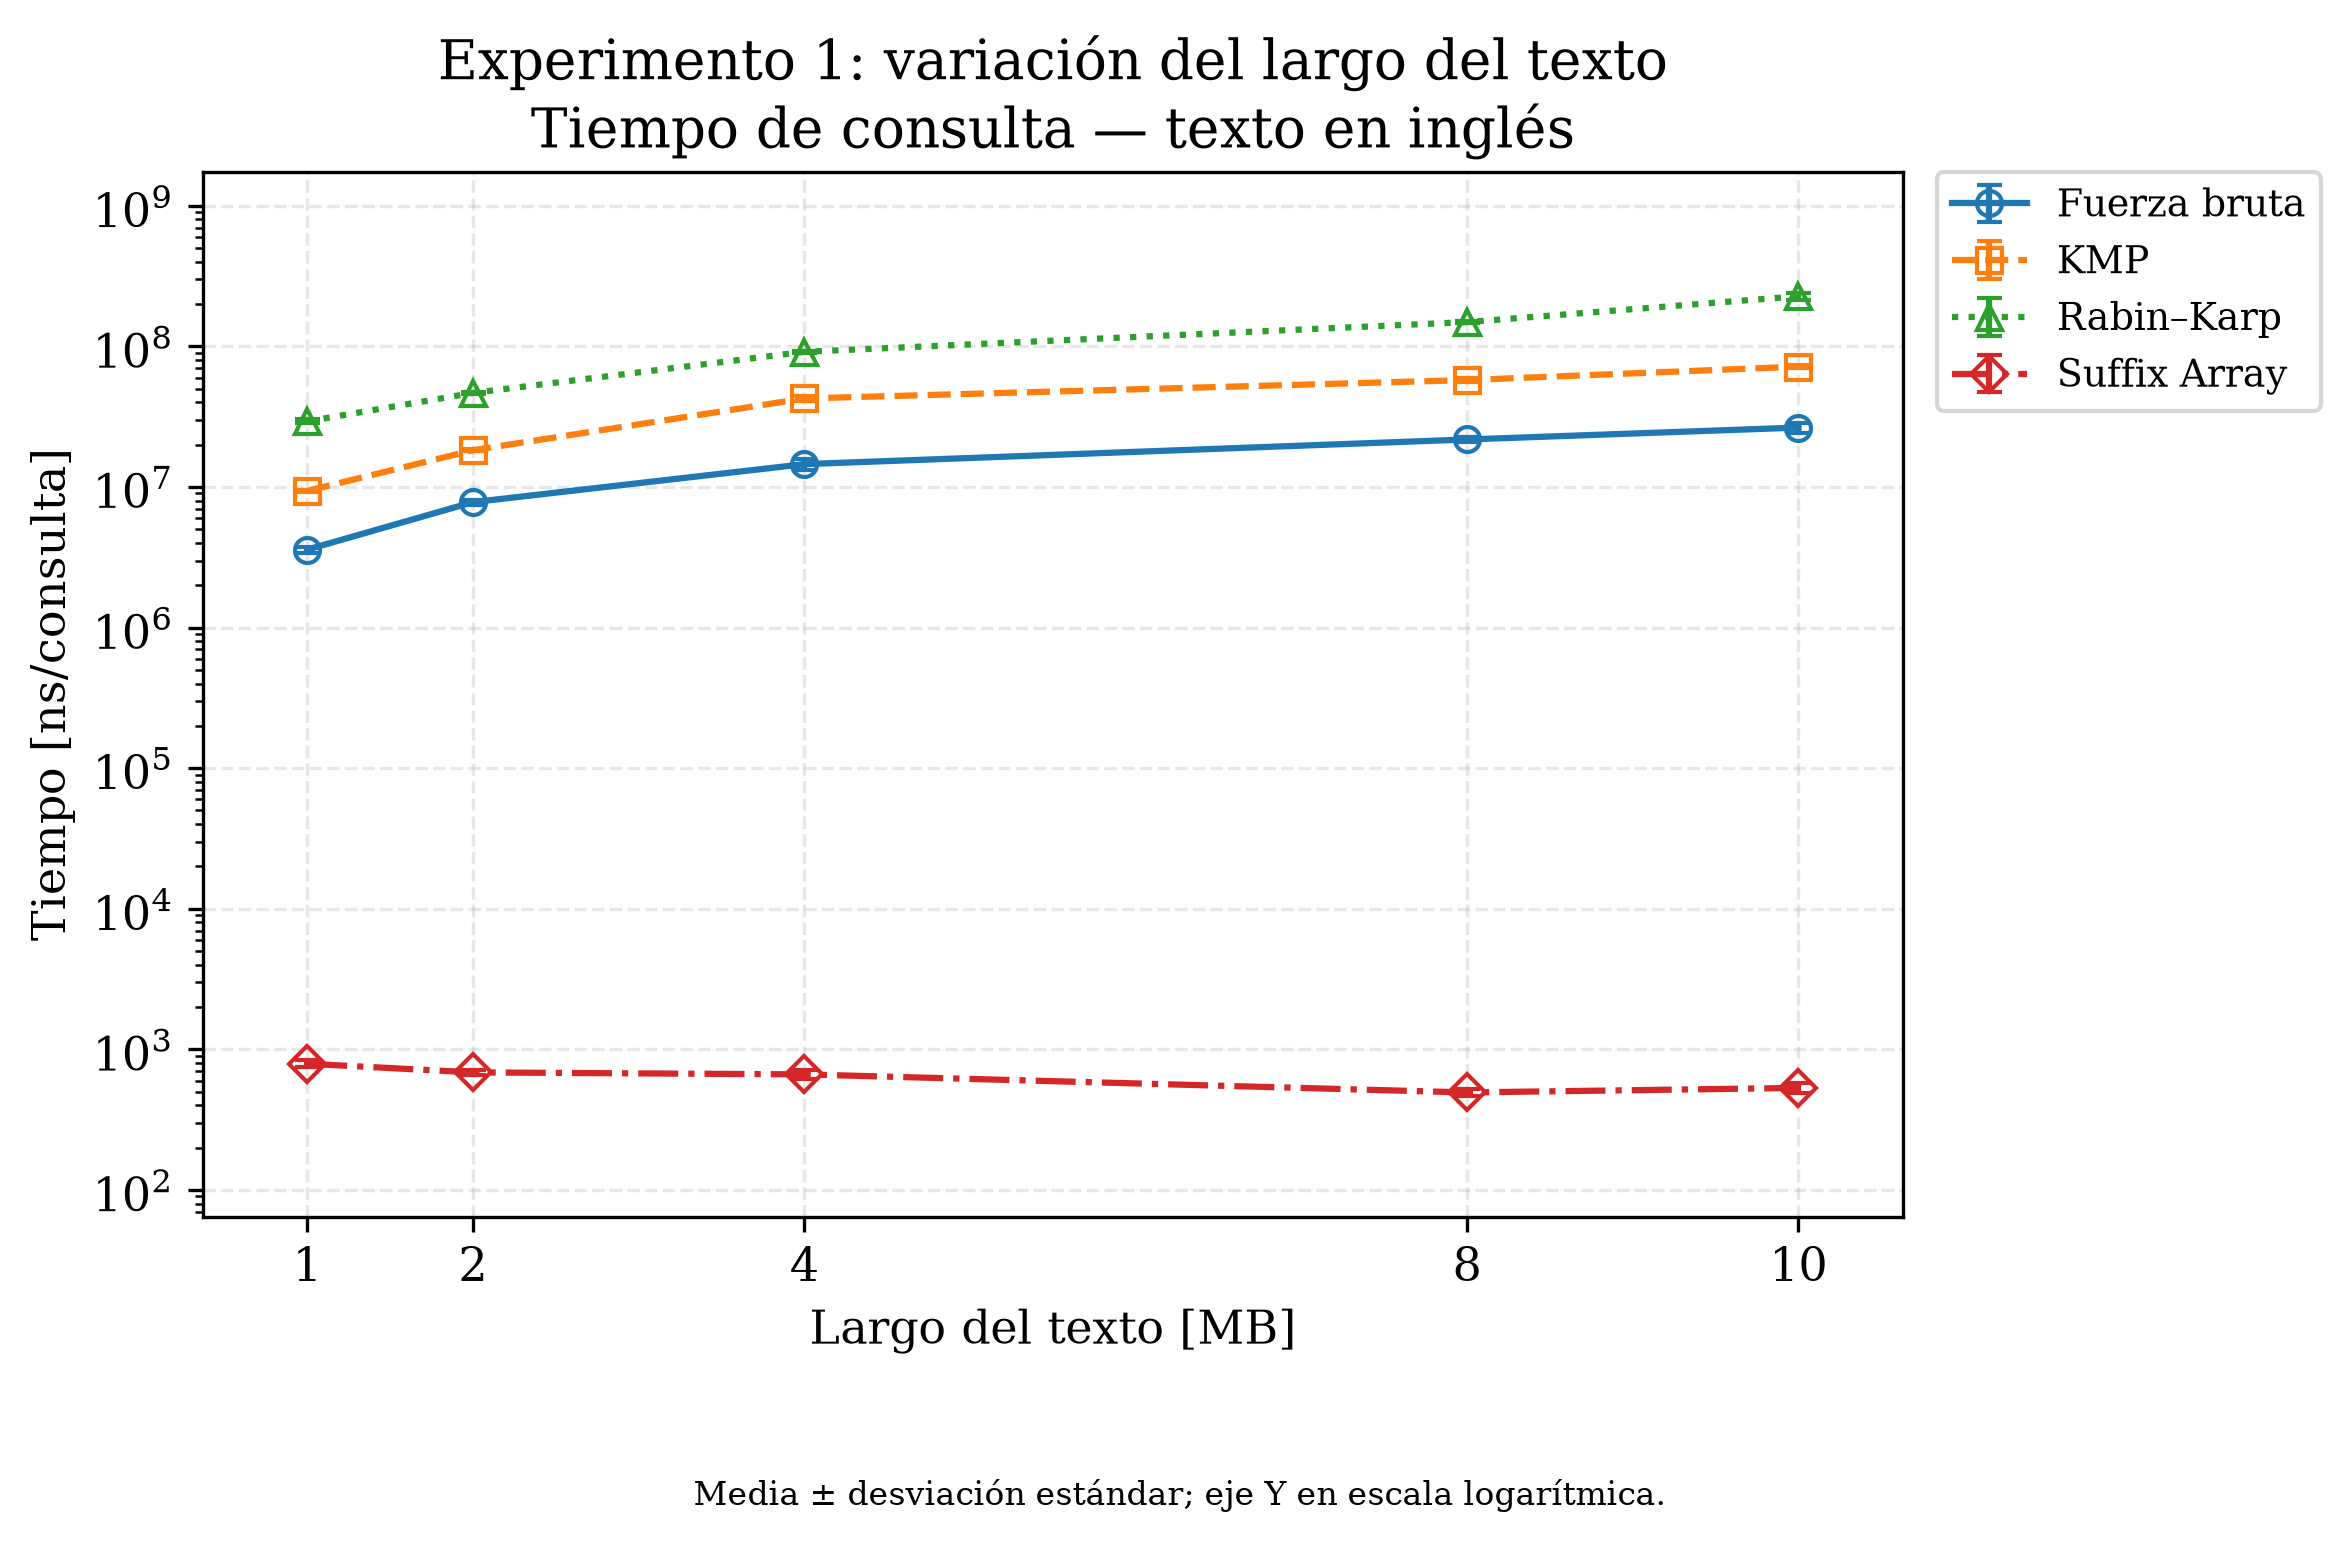
\includegraphics[width=\linewidth]{../plots/experimento_1_largo_texto/tiempo_consulta_vs_largo_texto.png}
        \caption{Tiempo de consulta.}
        \label{fig:res-texto-tiempo}
    \end{subfigure}\hfill
    \begin{subfigure}[t]{0.49\linewidth}
        \centering
        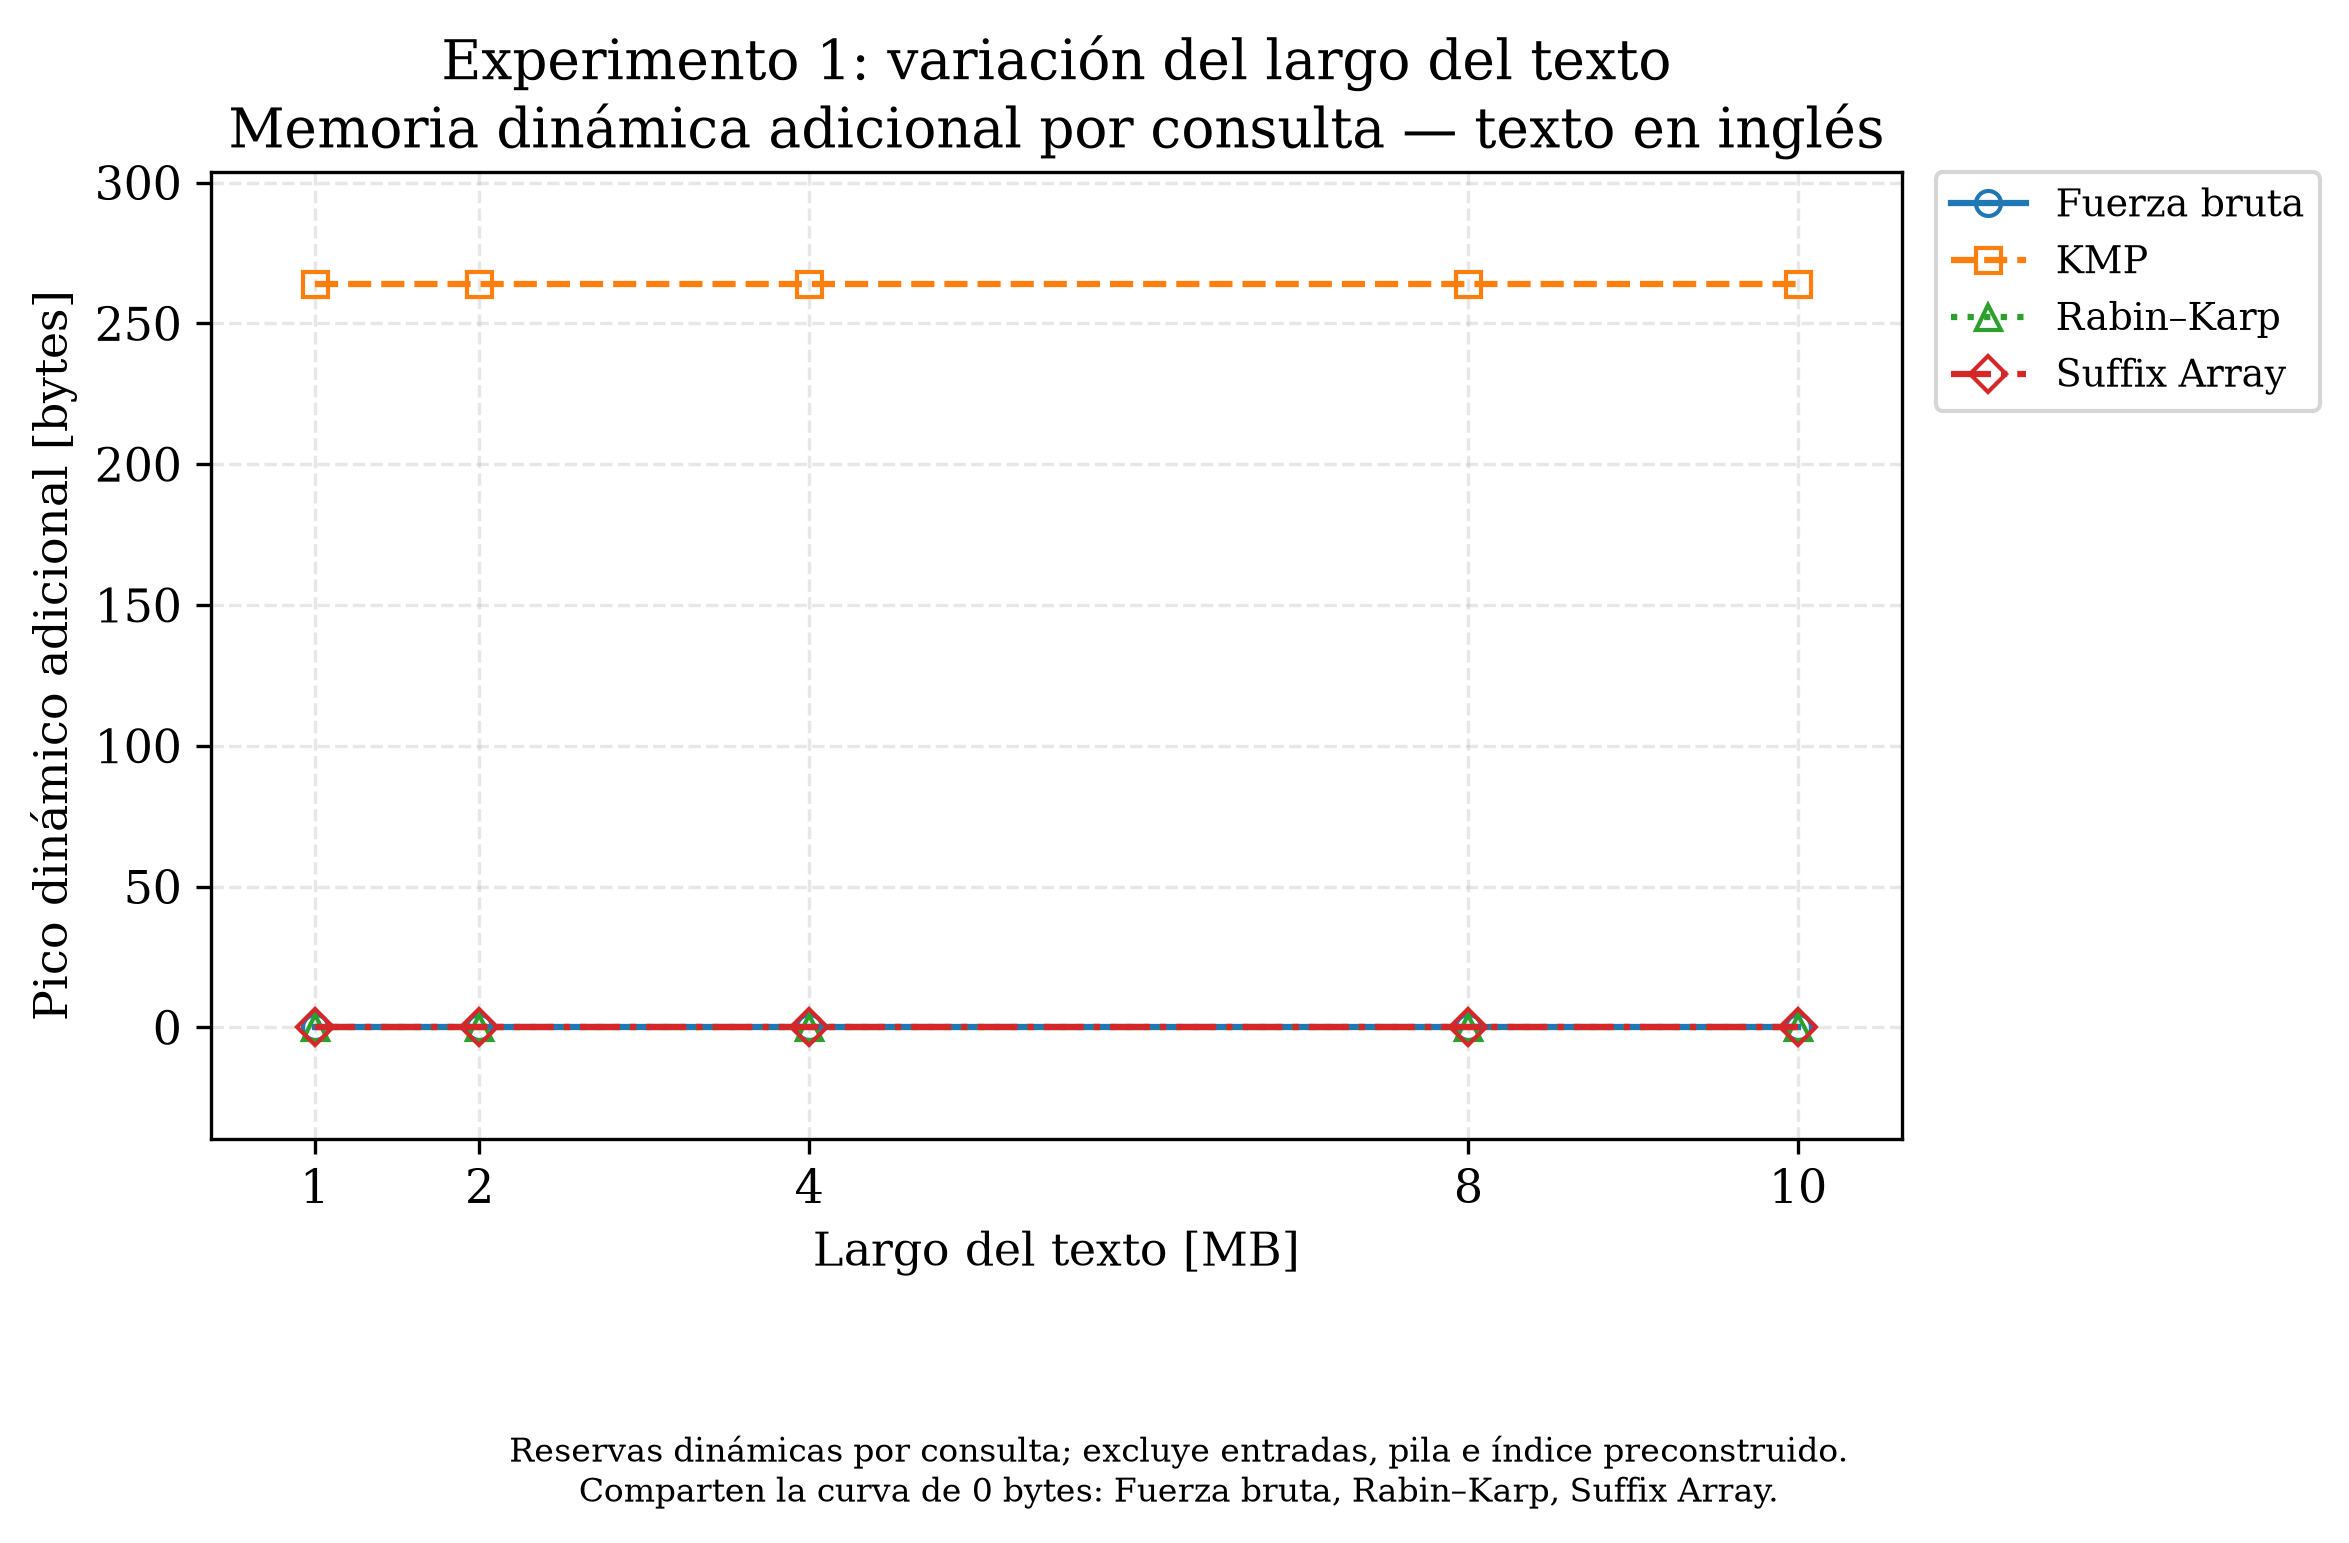
\includegraphics[width=\linewidth]{../plots/experimento_1_largo_texto/memoria_auxiliar_consulta_vs_largo_texto.png}
        \caption{Memoria auxiliar por consulta.}
        \label{fig:res-texto-memoria-consulta}
    \end{subfigure}

    \par\medskip
    \begin{subfigure}[t]{0.49\linewidth}
        \centering
        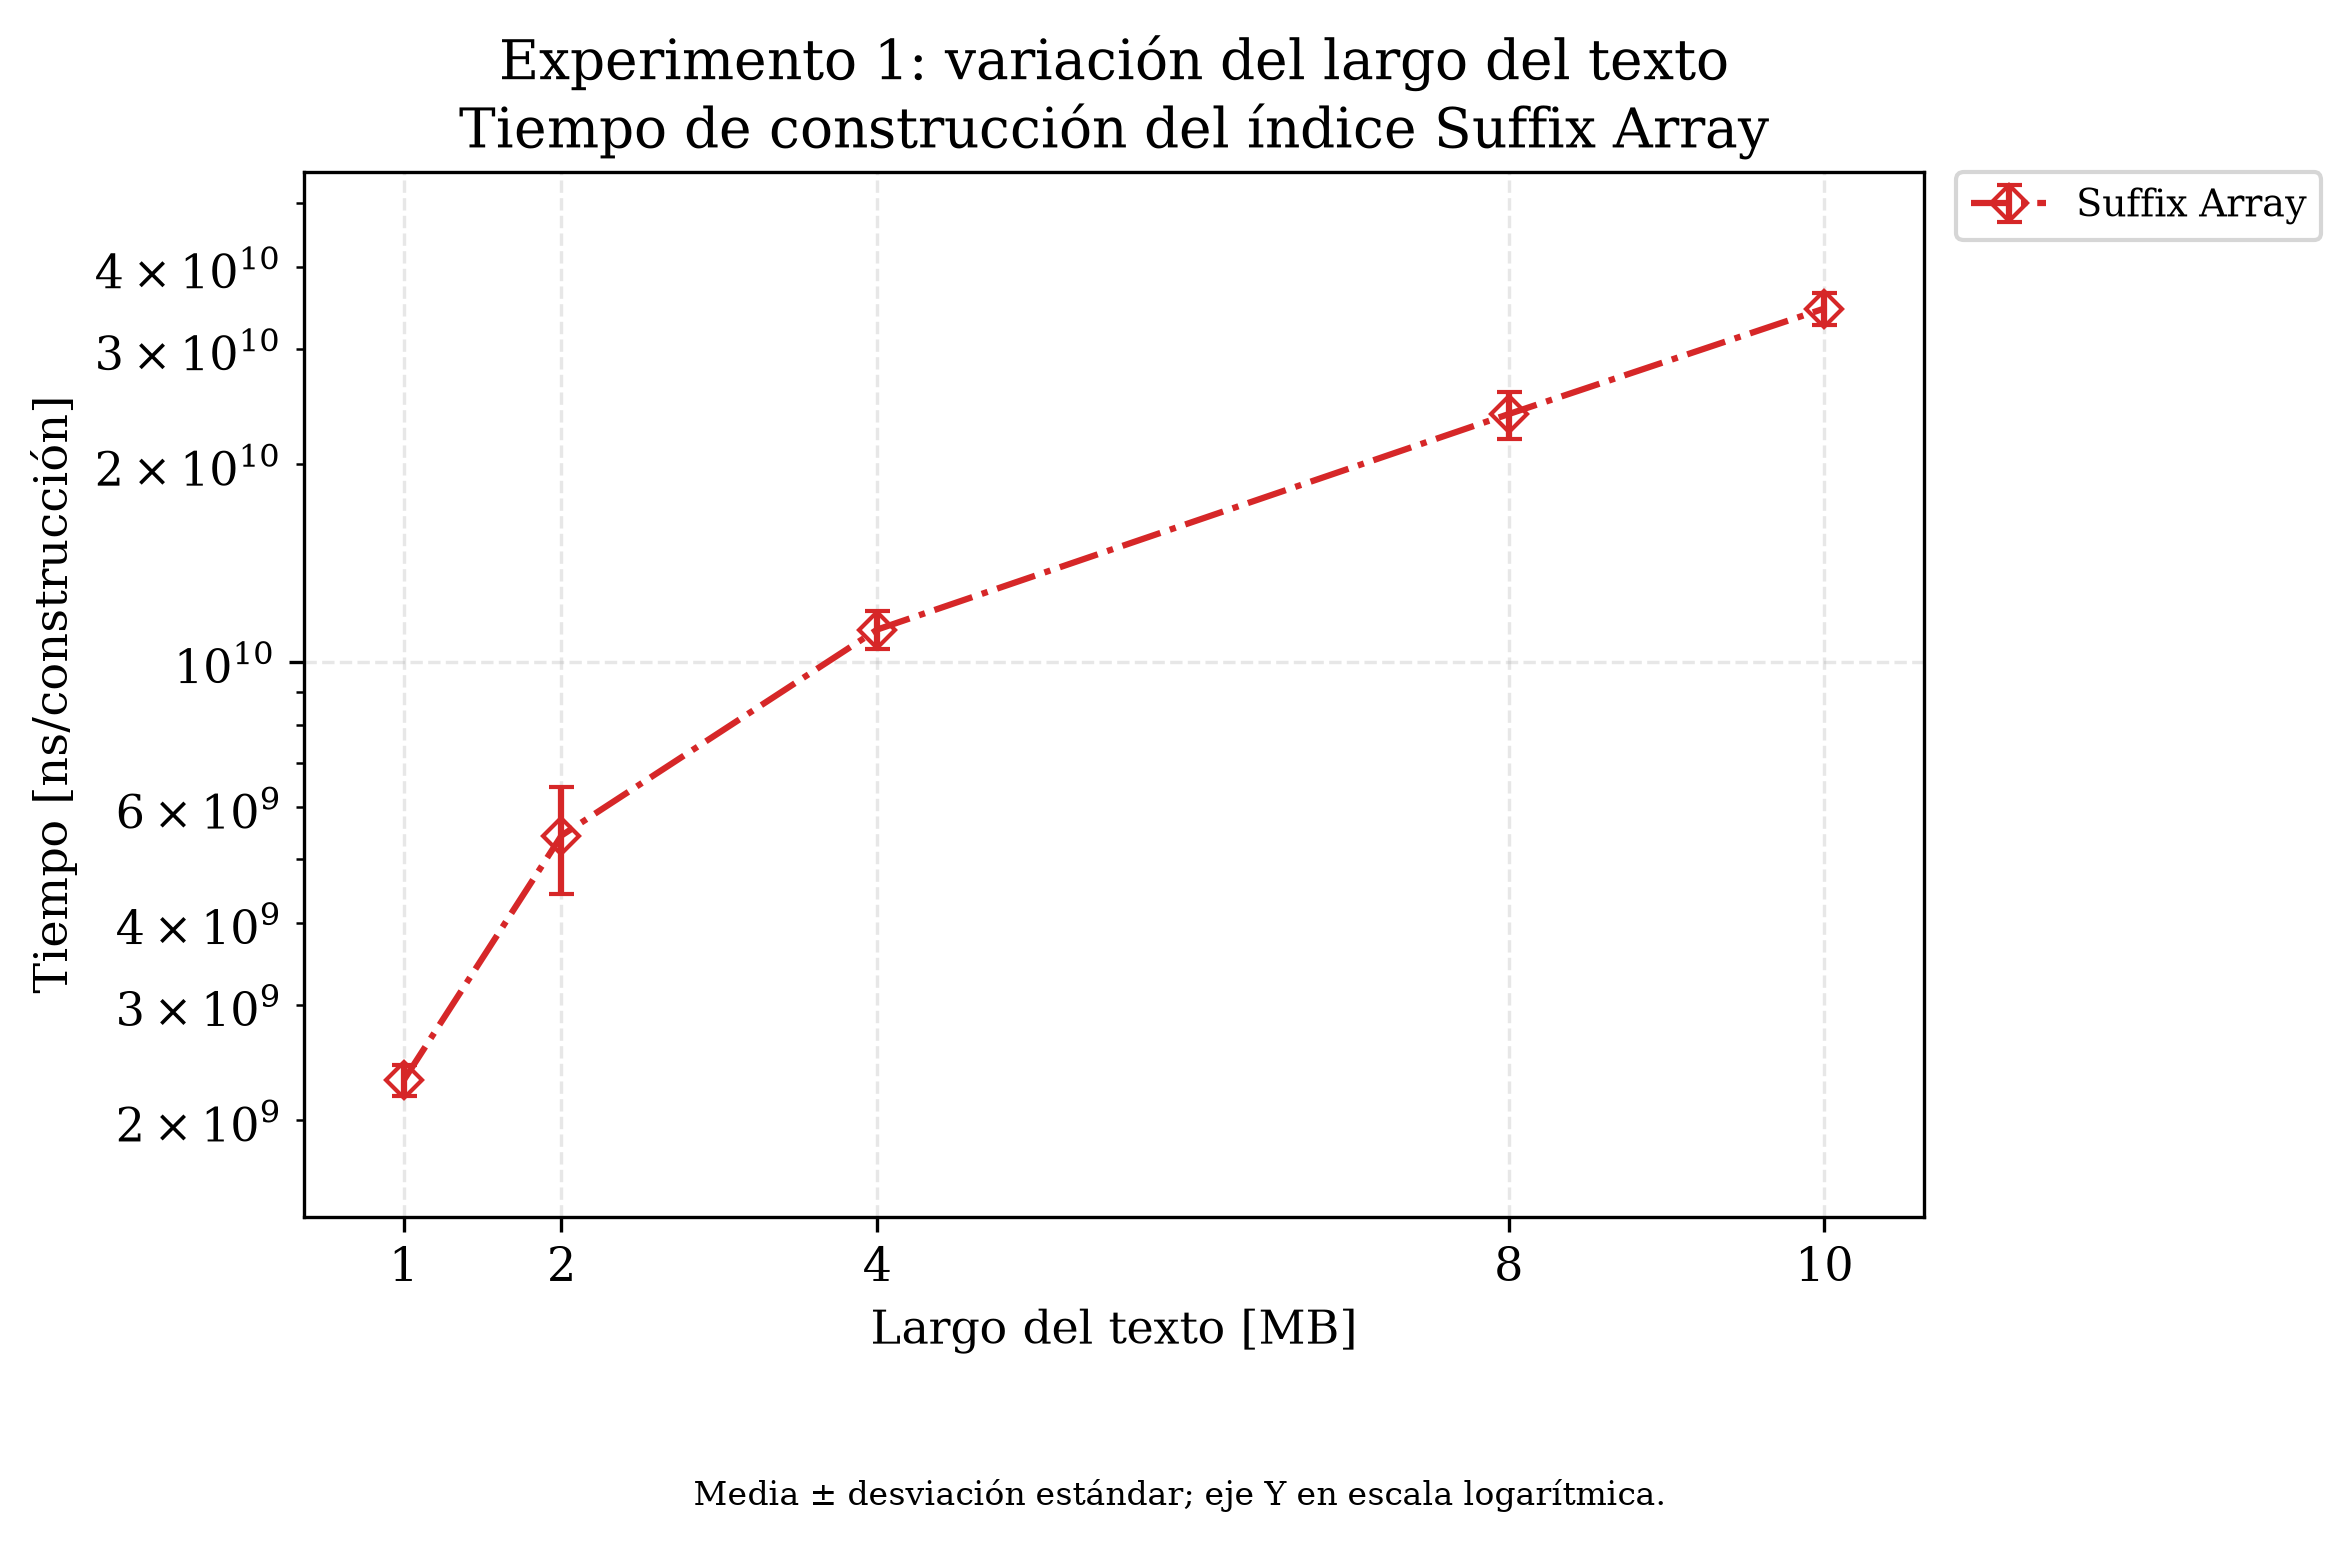
\includegraphics[width=\linewidth]{../plots/experimento_1_largo_texto/tiempo_construccion_suffix_array_vs_largo_texto.png}
        \caption{Tiempo de construcción.}
        \label{fig:res-texto-construccion}
    \end{subfigure}\hfill
    \begin{subfigure}[t]{0.49\linewidth}
        \centering
        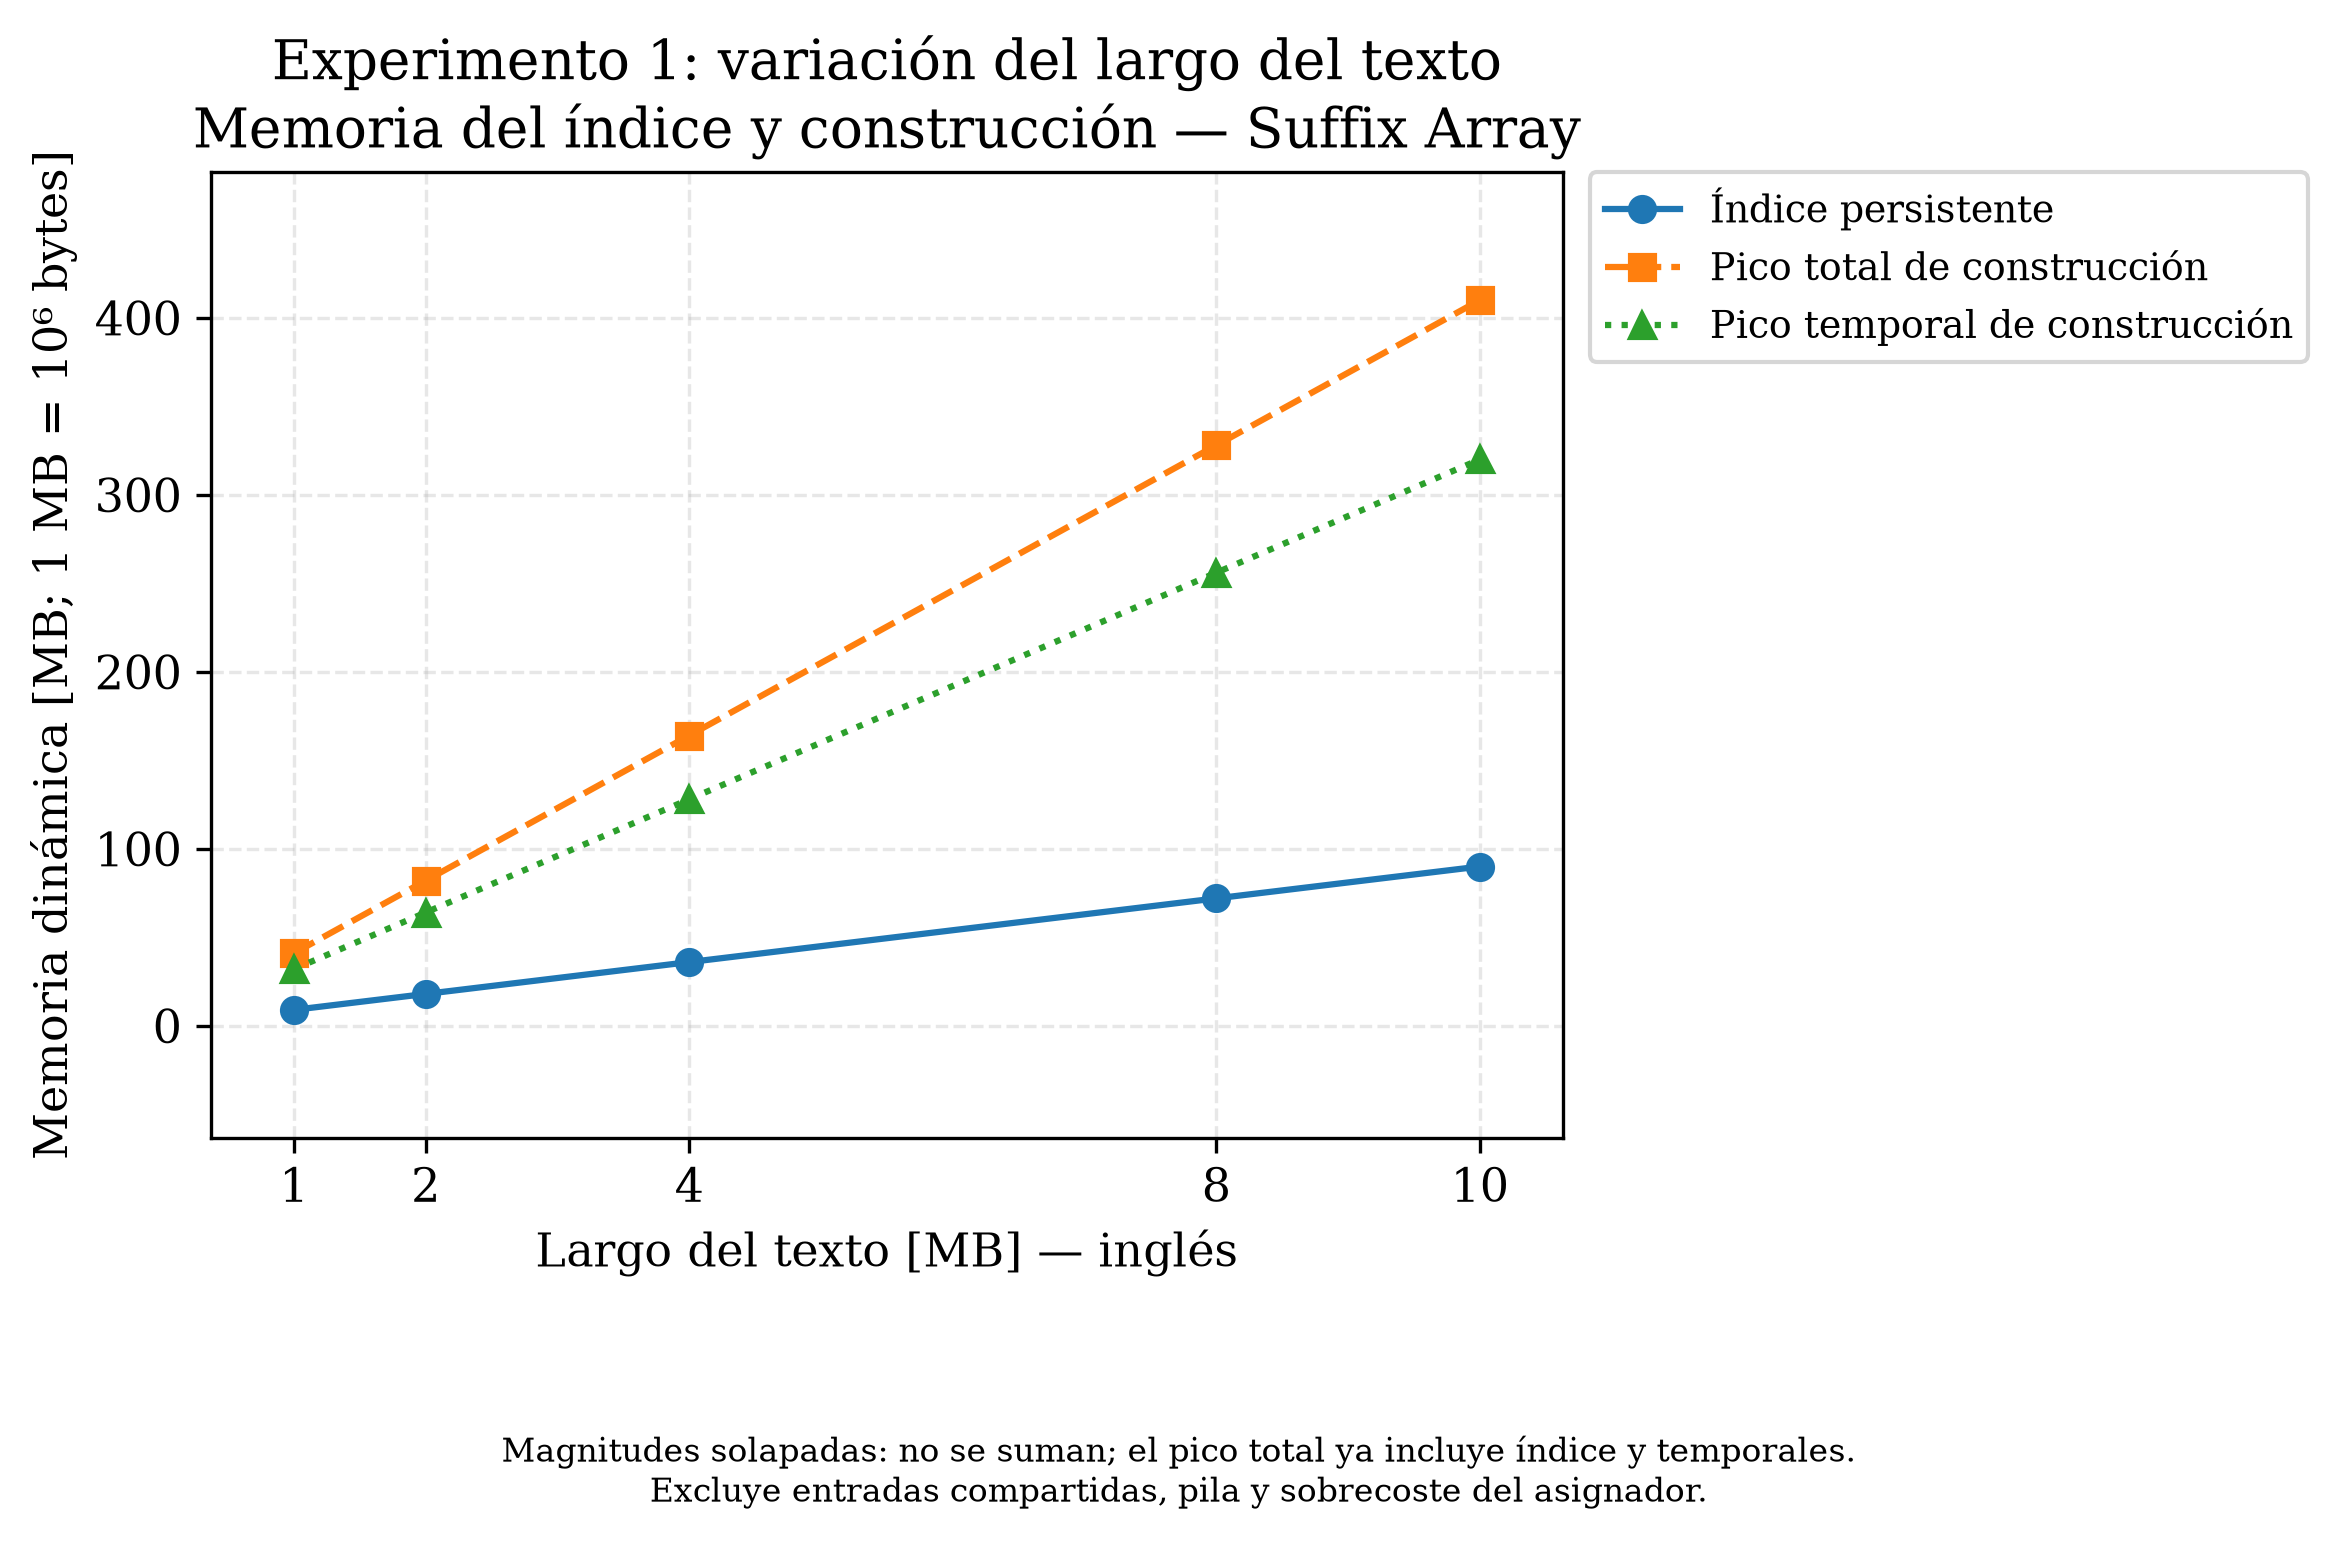
\includegraphics[width=\linewidth]{../plots/experimento_1_largo_texto/memoria_indice_y_construccion_suffix_array_vs_largo_texto.png}
        \caption{Memoria del índice y construcción.}
        \label{fig:res-texto-memoria-indice}
    \end{subfigure}
    \caption{Experimento 1: largo del texto.}
    \label{fig:res-experimento-1}
\end{figure}

\clearpage
\subsection{Experimento 2: largo del patrón}

\begin{figure}[!ht]
    \centering
    \begin{subfigure}[t]{0.49\linewidth}
        \centering
        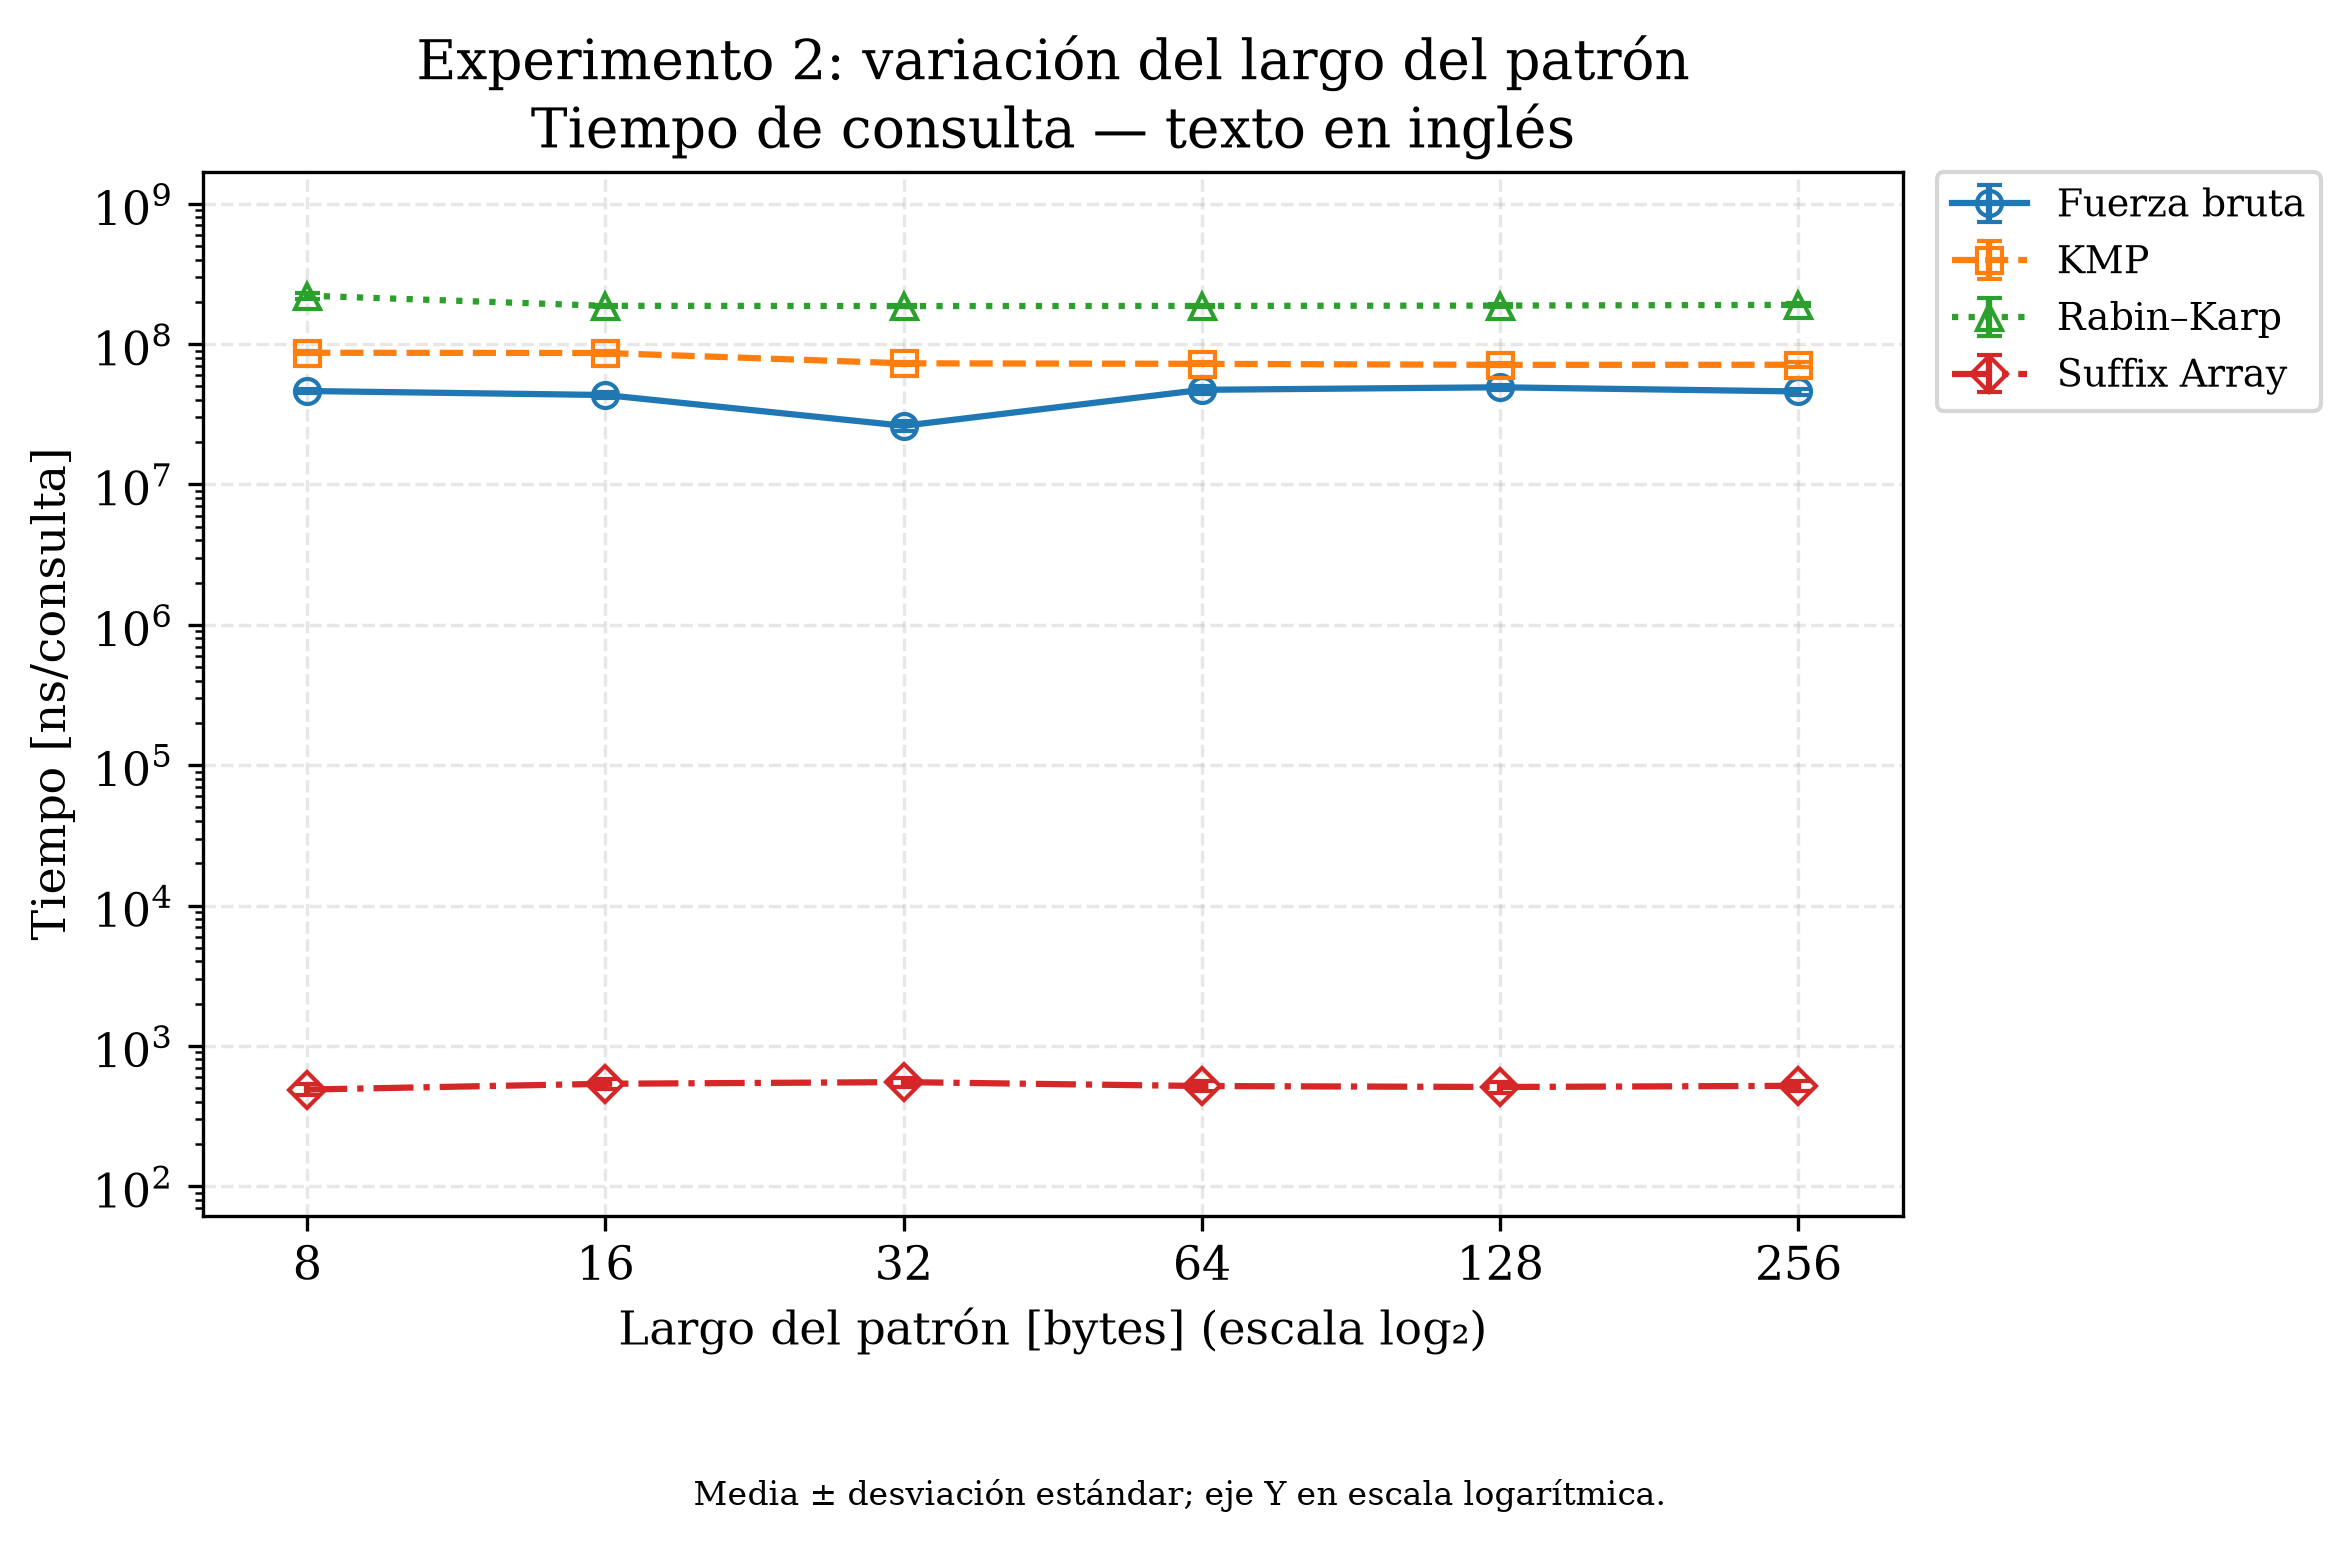
\includegraphics[width=\linewidth]{../plots/experimento_2_largo_patron/tiempo_consulta_vs_largo_patron.png}
        \caption{Tiempo de consulta.}
        \label{fig:res-patron-tiempo}
    \end{subfigure}\hfill
    \begin{subfigure}[t]{0.49\linewidth}
        \centering
        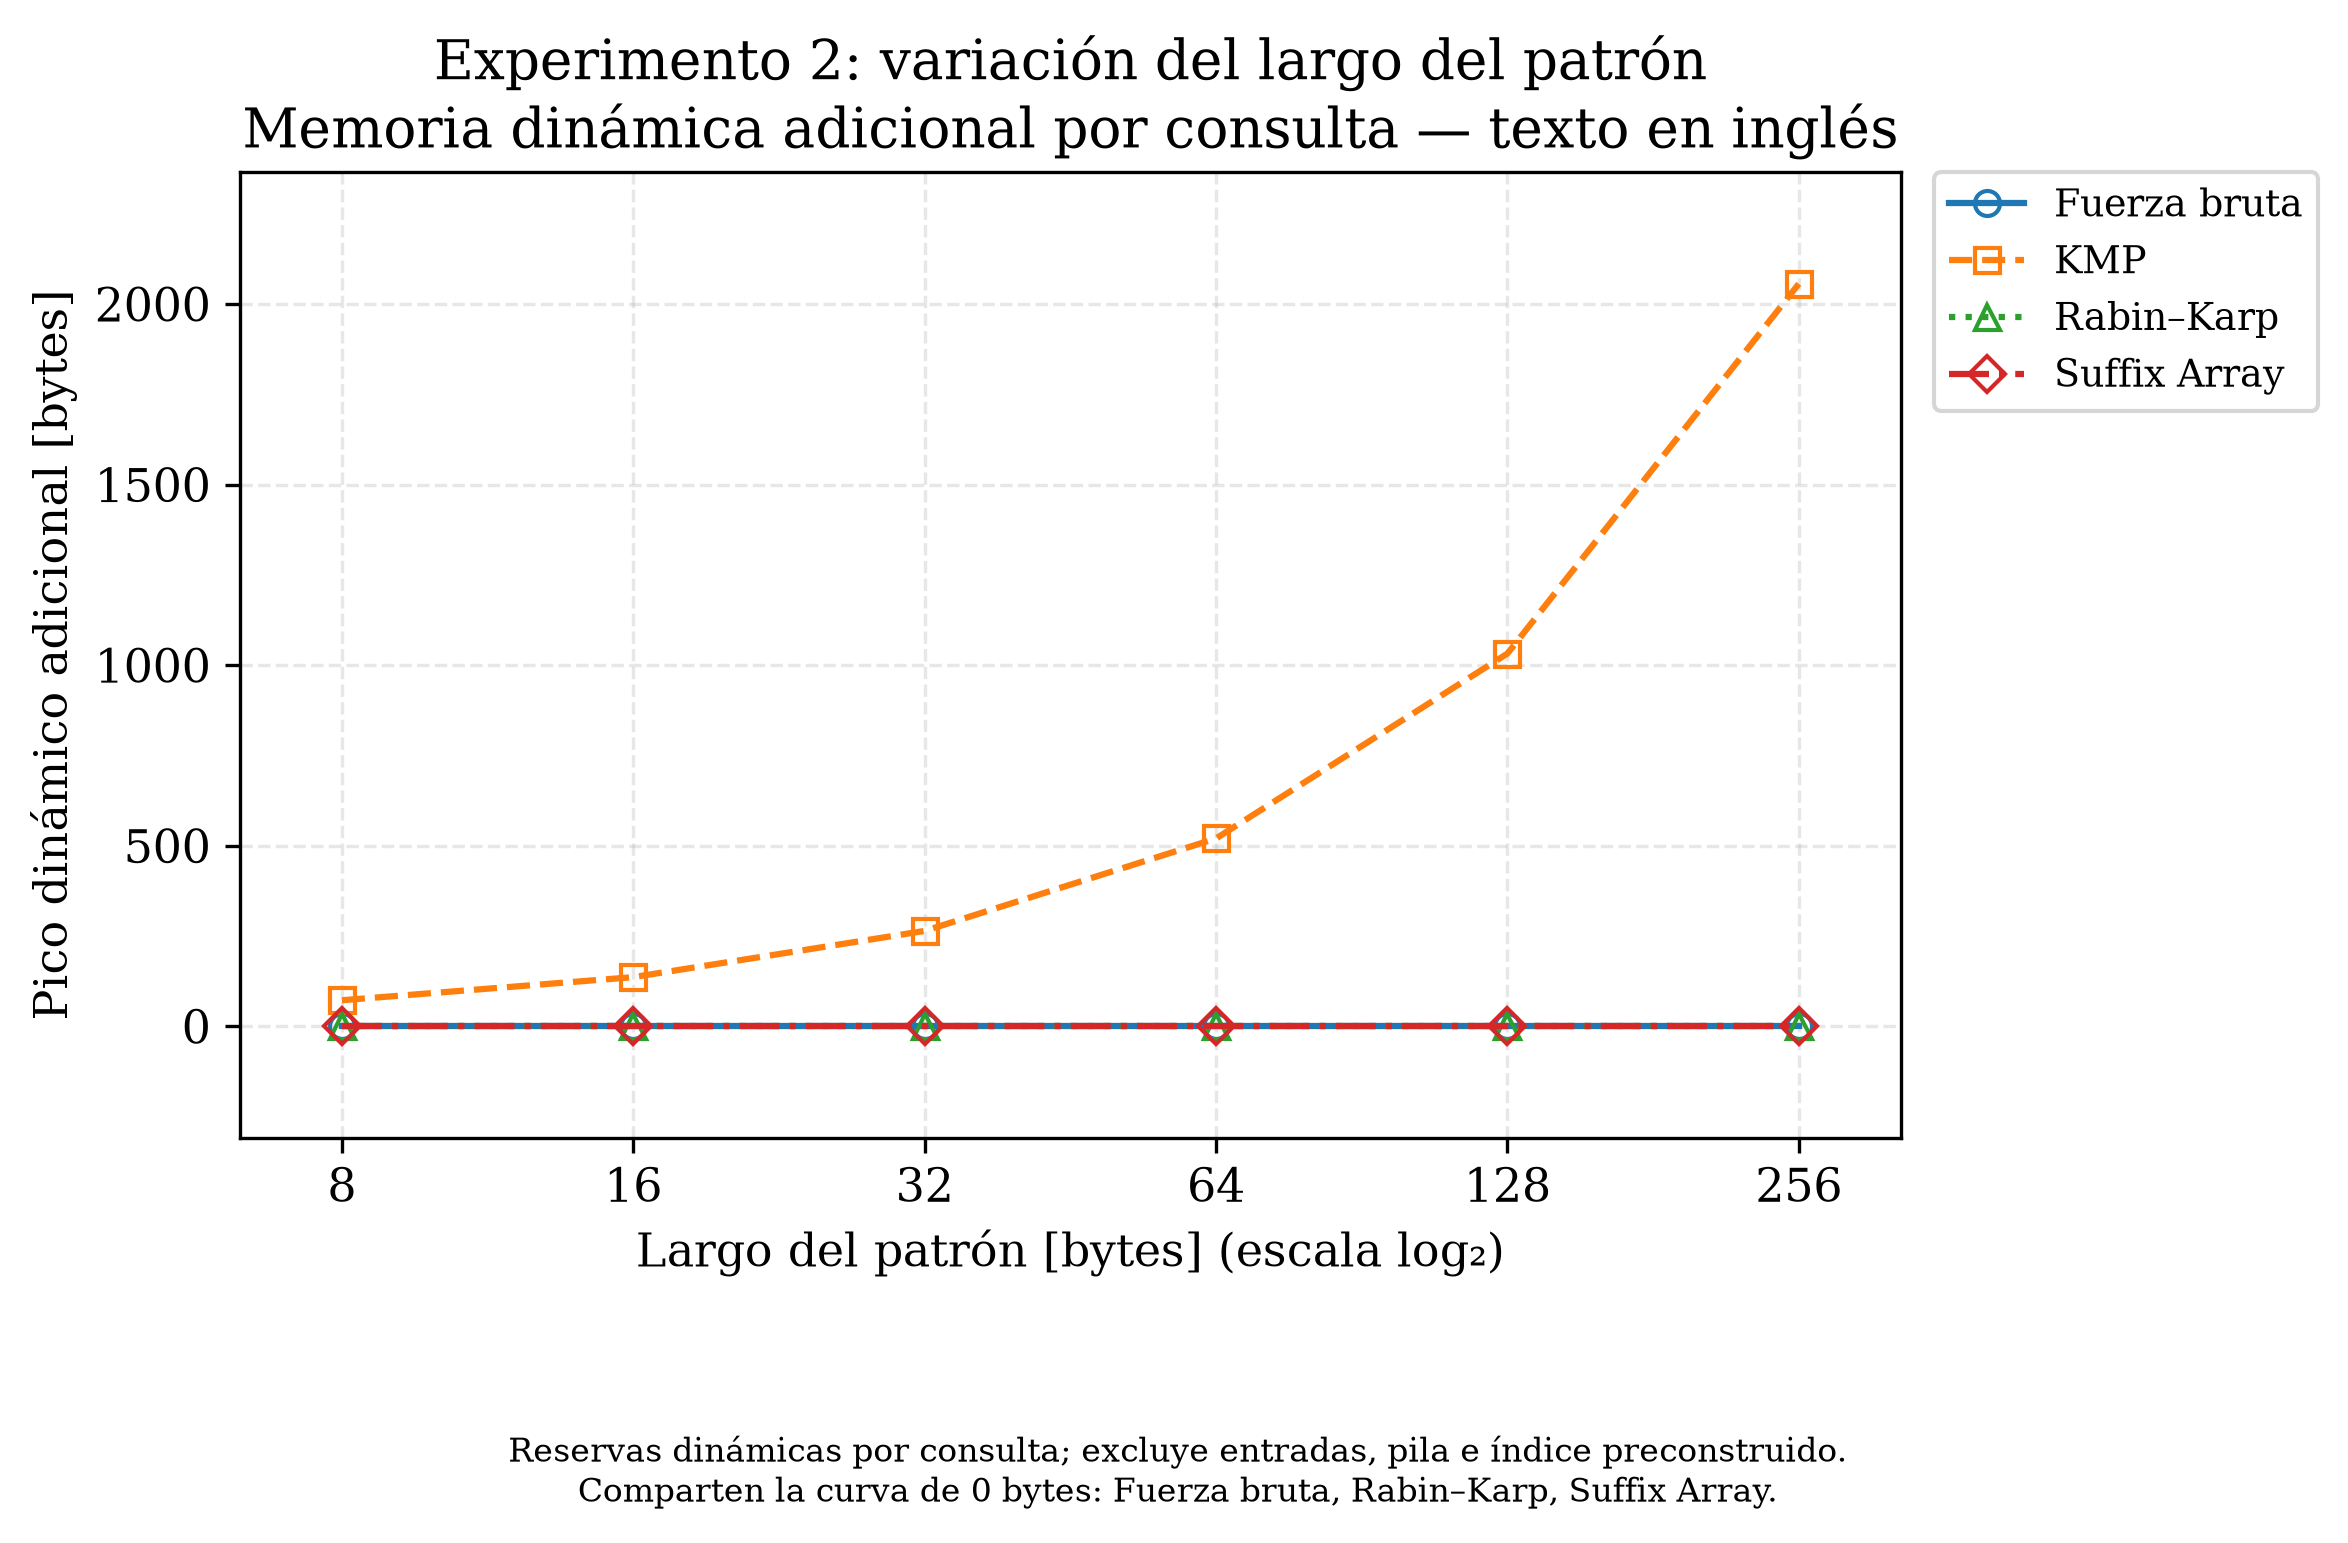
\includegraphics[width=\linewidth]{../plots/experimento_2_largo_patron/memoria_auxiliar_consulta_vs_largo_patron.png}
        \caption{Memoria auxiliar por consulta.}
        \label{fig:res-patron-memoria-consulta}
    \end{subfigure}

    \par\medskip
    \begin{subfigure}[t]{0.58\linewidth}
        \centering
        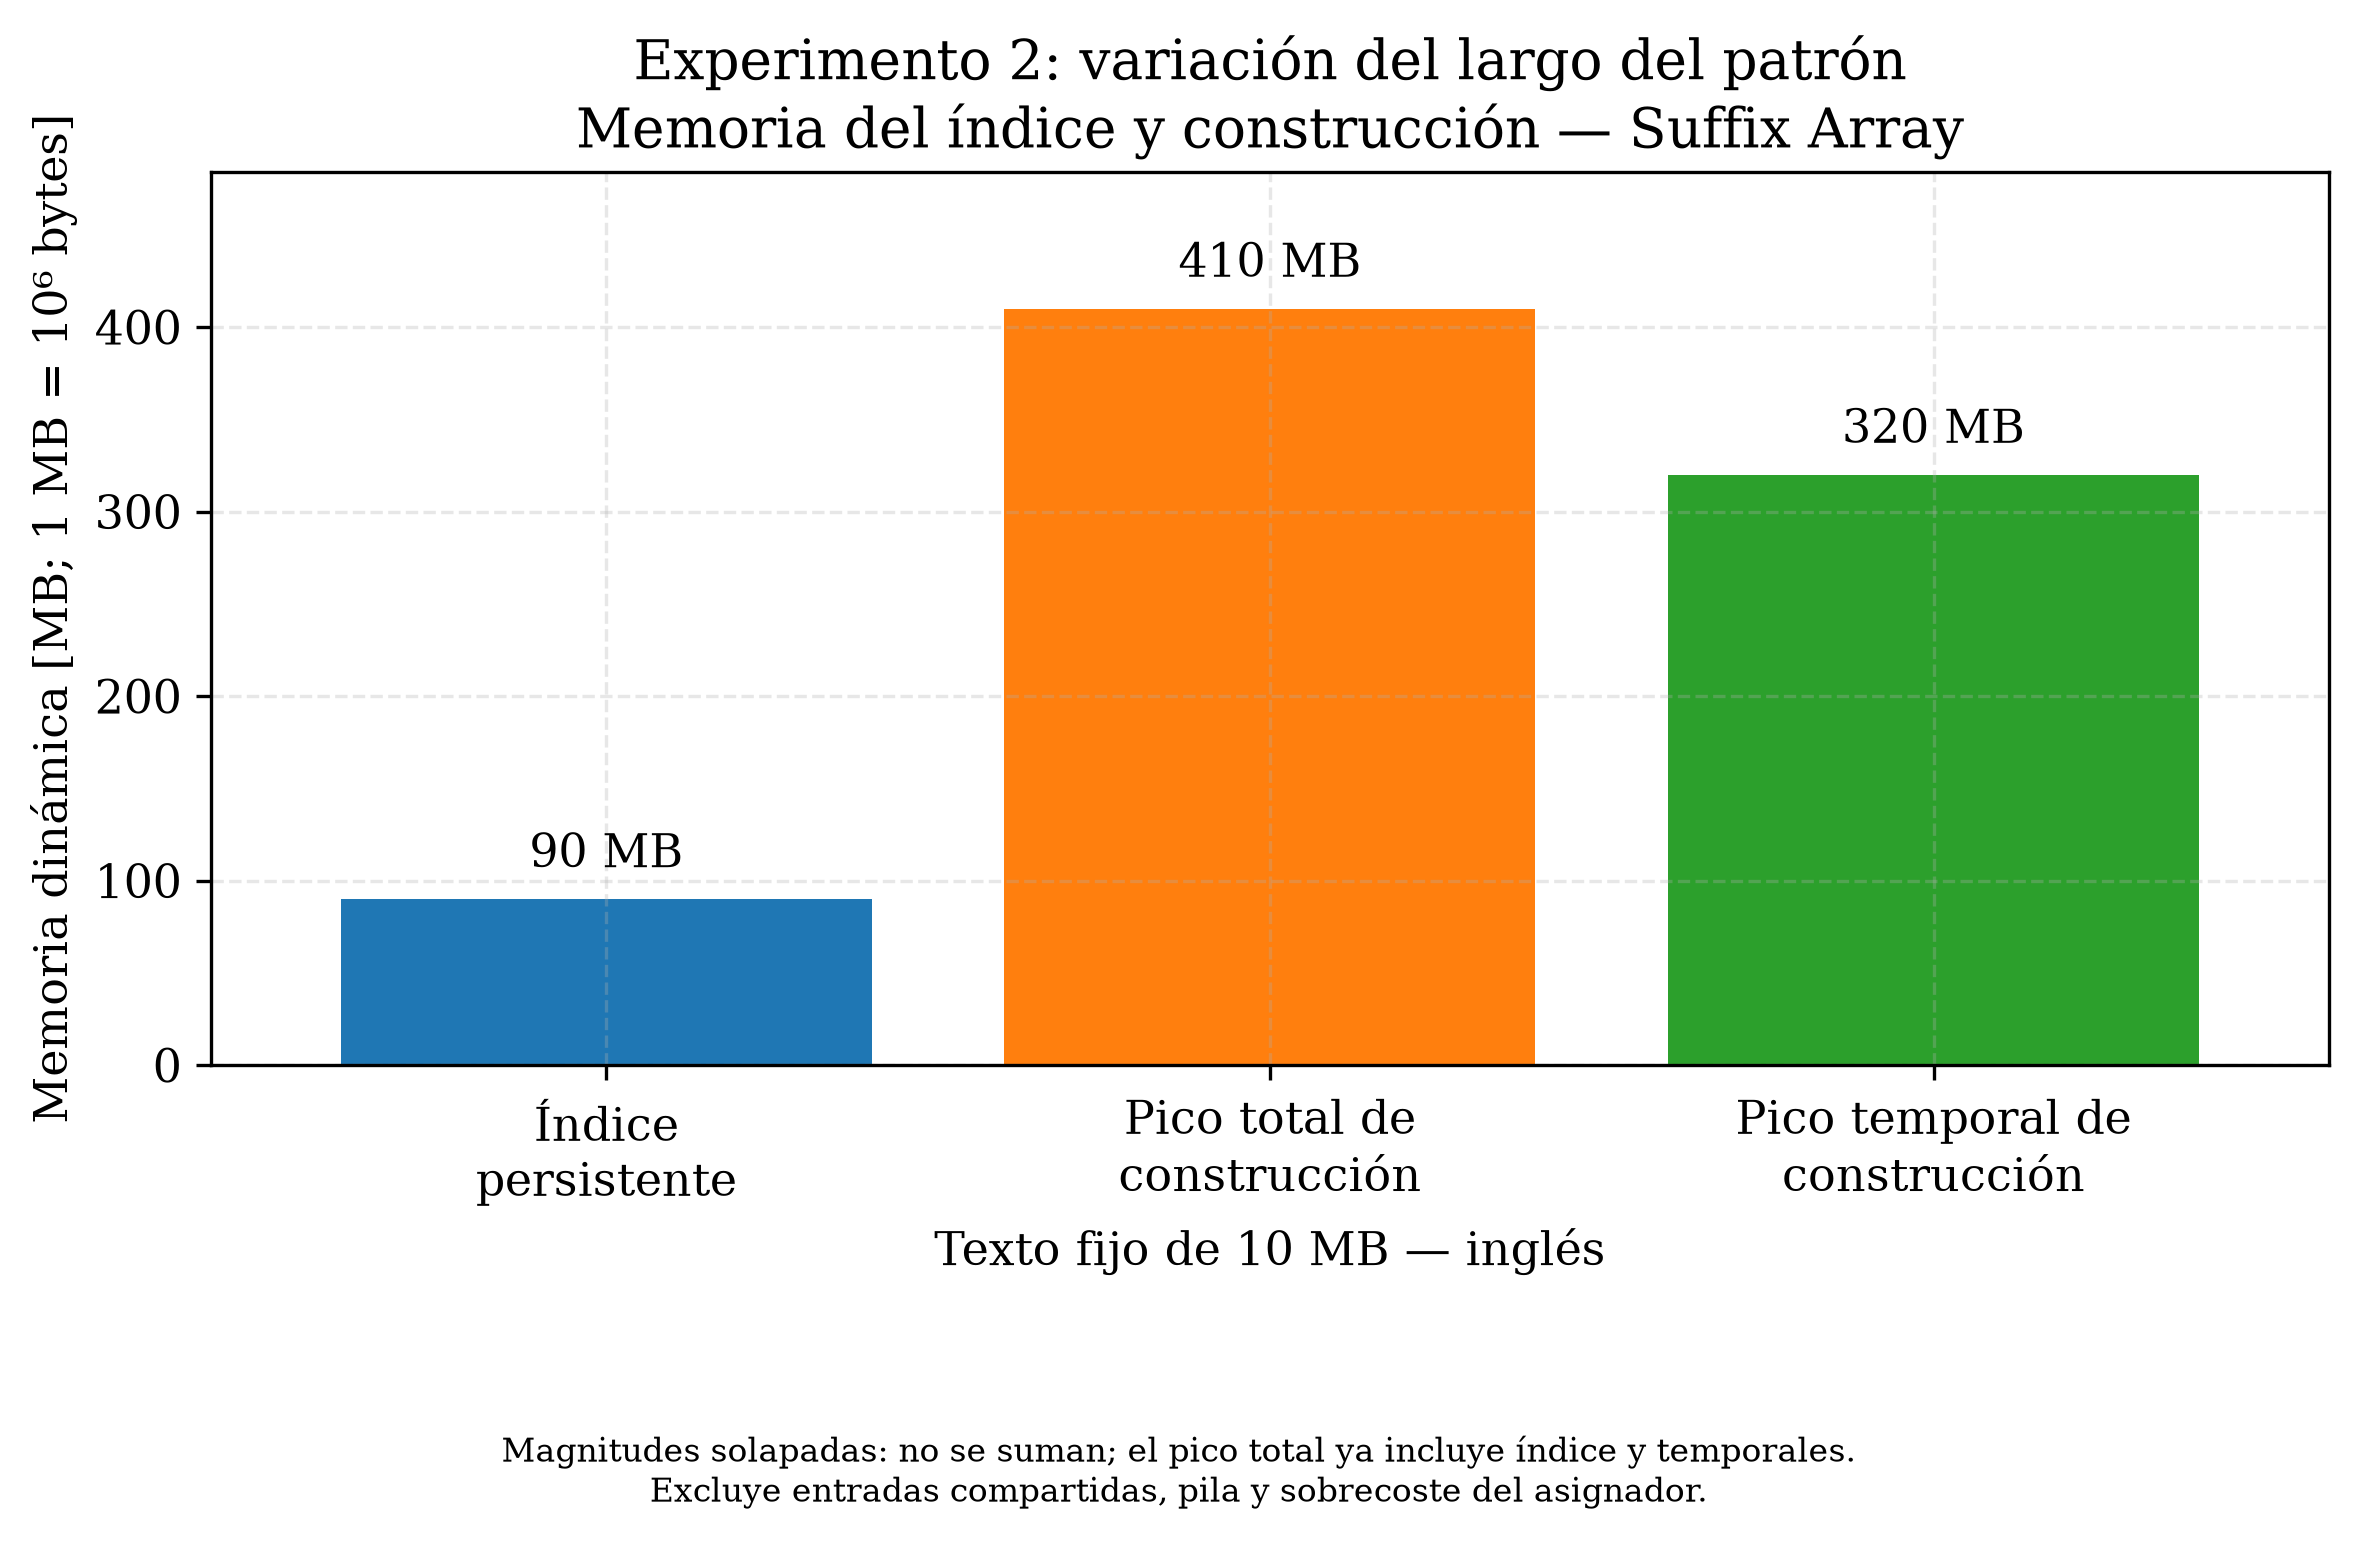
\includegraphics[width=\linewidth]{../plots/experimento_2_largo_patron/memoria_indice_y_construccion_suffix_array_texto_fijo.png}
        \caption{Memoria del índice y construcción.}
        \label{fig:res-patron-memoria-indice}
    \end{subfigure}
    \caption{Experimento 2: largo del patrón.}
    \label{fig:res-experimento-2}
\end{figure}

\clearpage
\subsection{Experimento 3: número de ocurrencias}

\begin{figure}[!ht]
    \centering
    \begin{subfigure}[t]{0.49\linewidth}
        \centering
        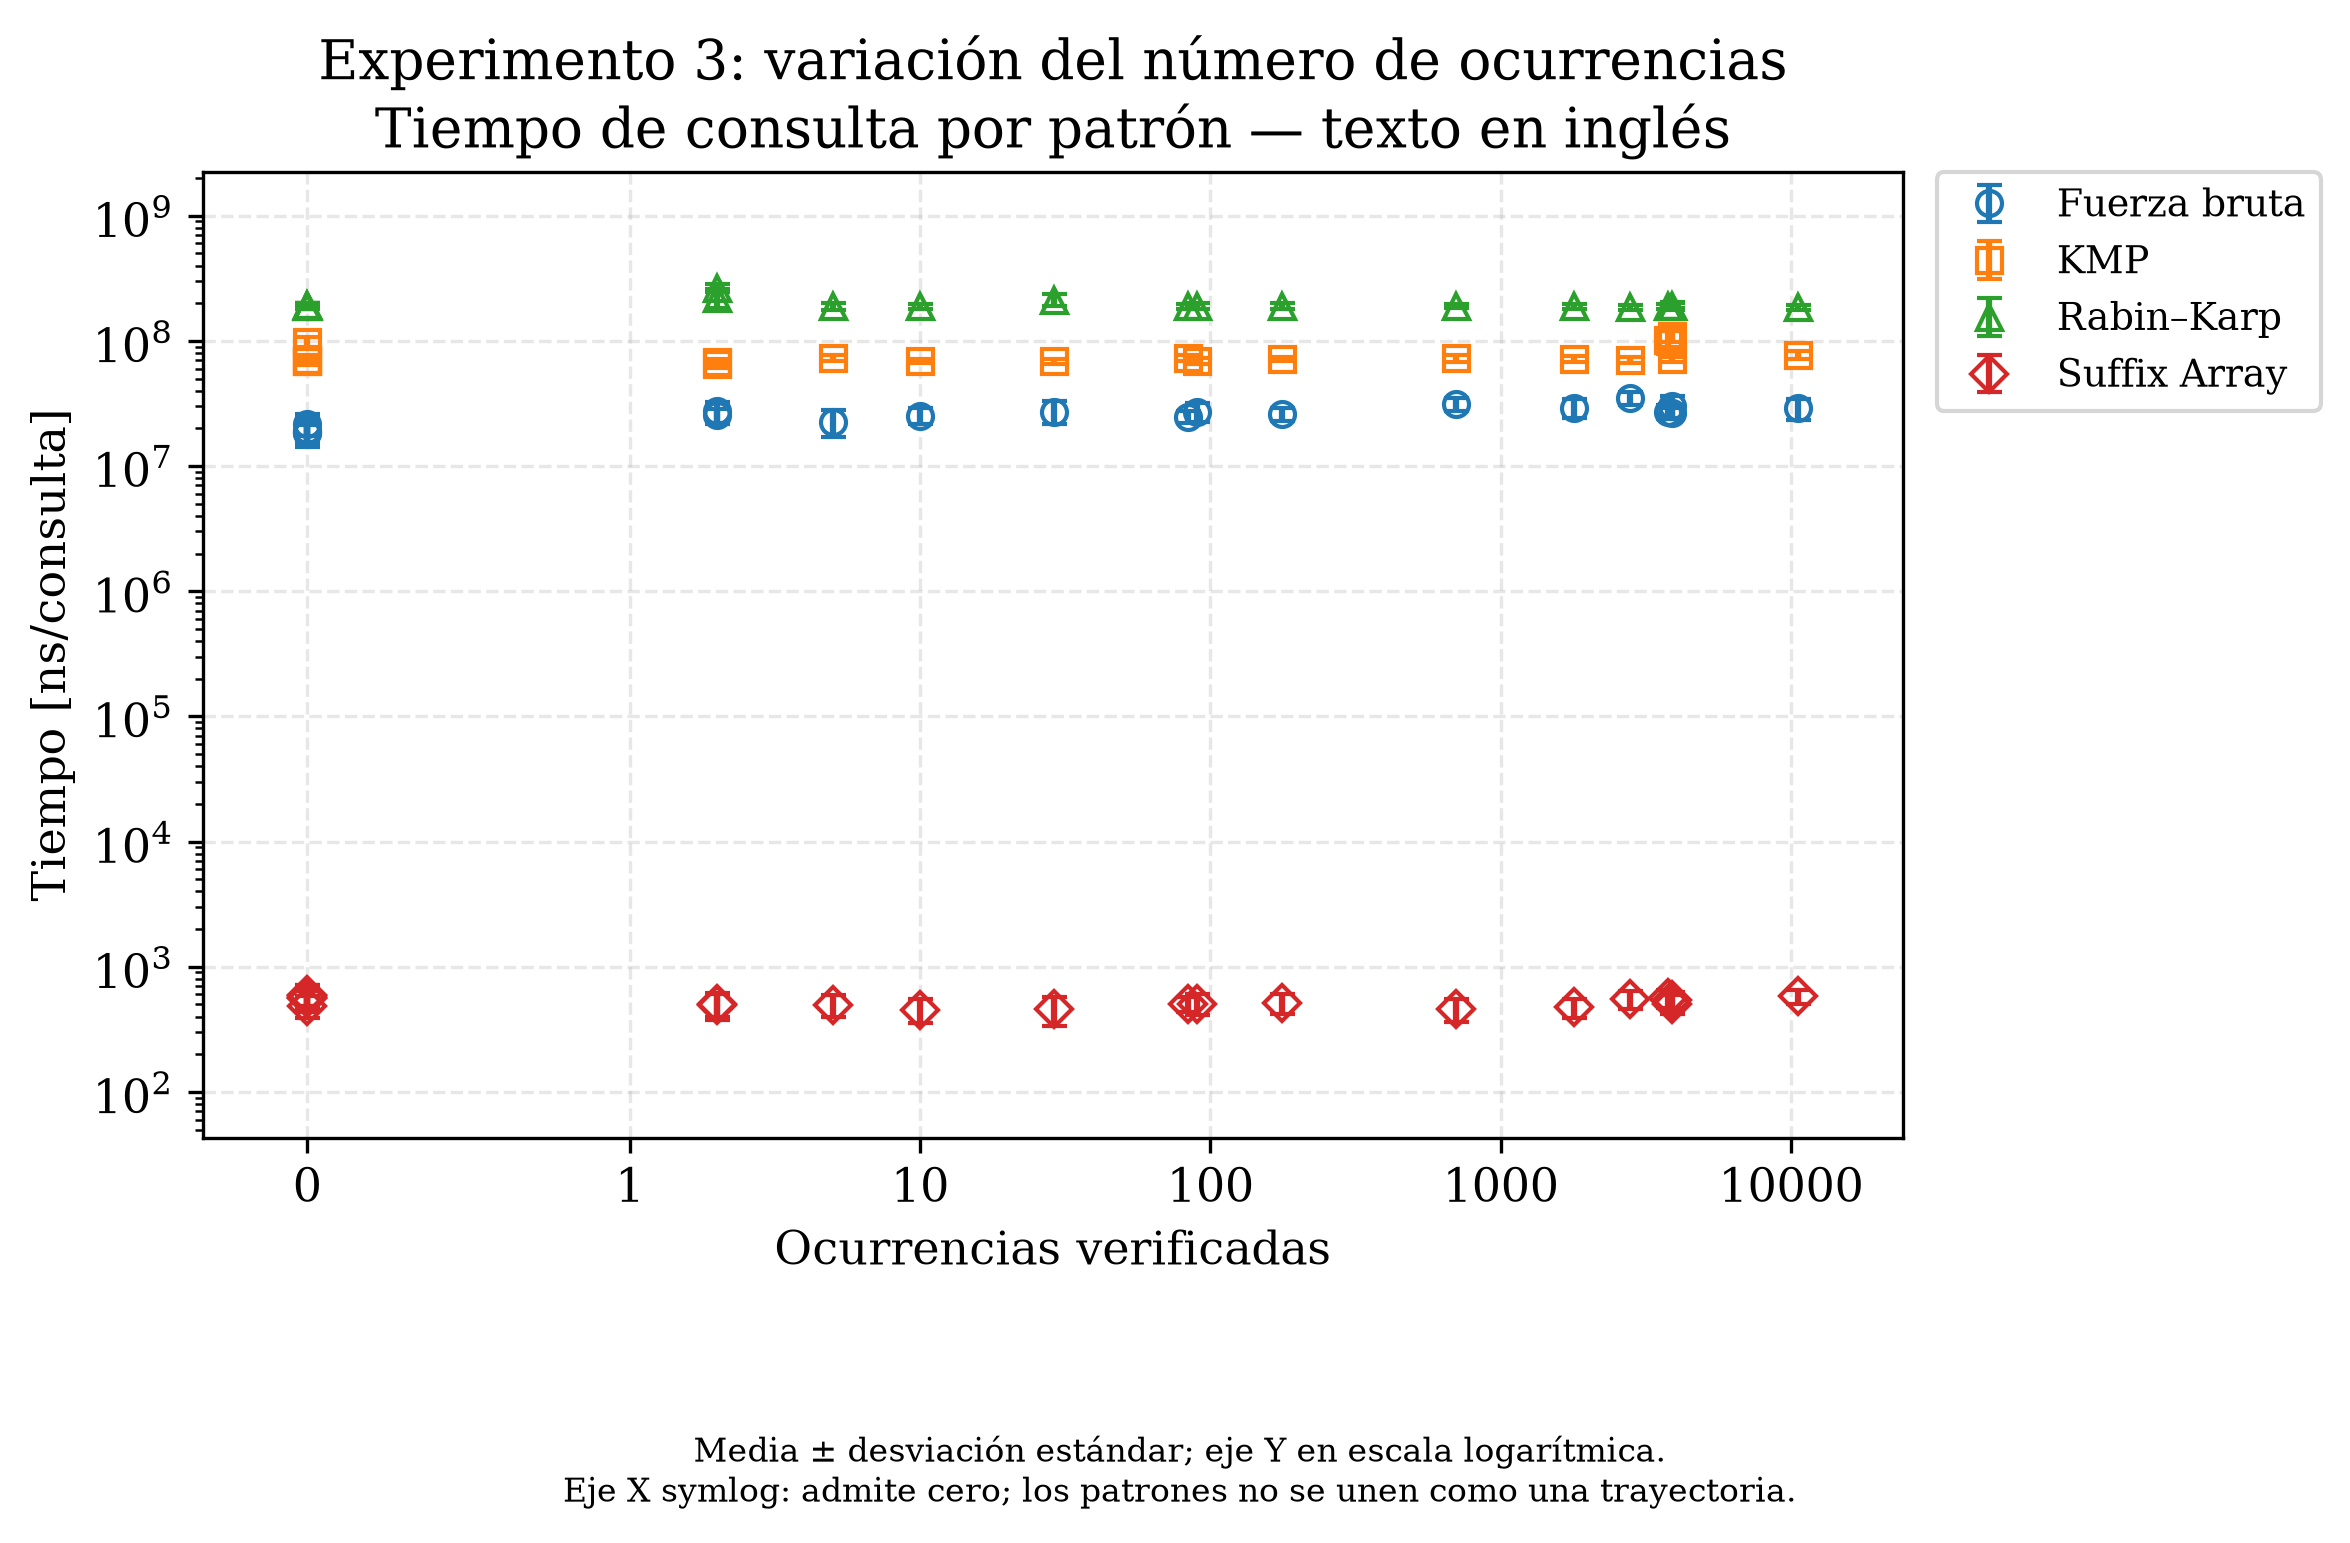
\includegraphics[width=\linewidth]{../plots/experimento_3_numero_ocurrencias/tiempo_consulta_vs_numero_ocurrencias.png}
        \caption{Tiempo de consulta.}
        \label{fig:res-ocurrencias-tiempo}
    \end{subfigure}\hfill
    \begin{subfigure}[t]{0.49\linewidth}
        \centering
        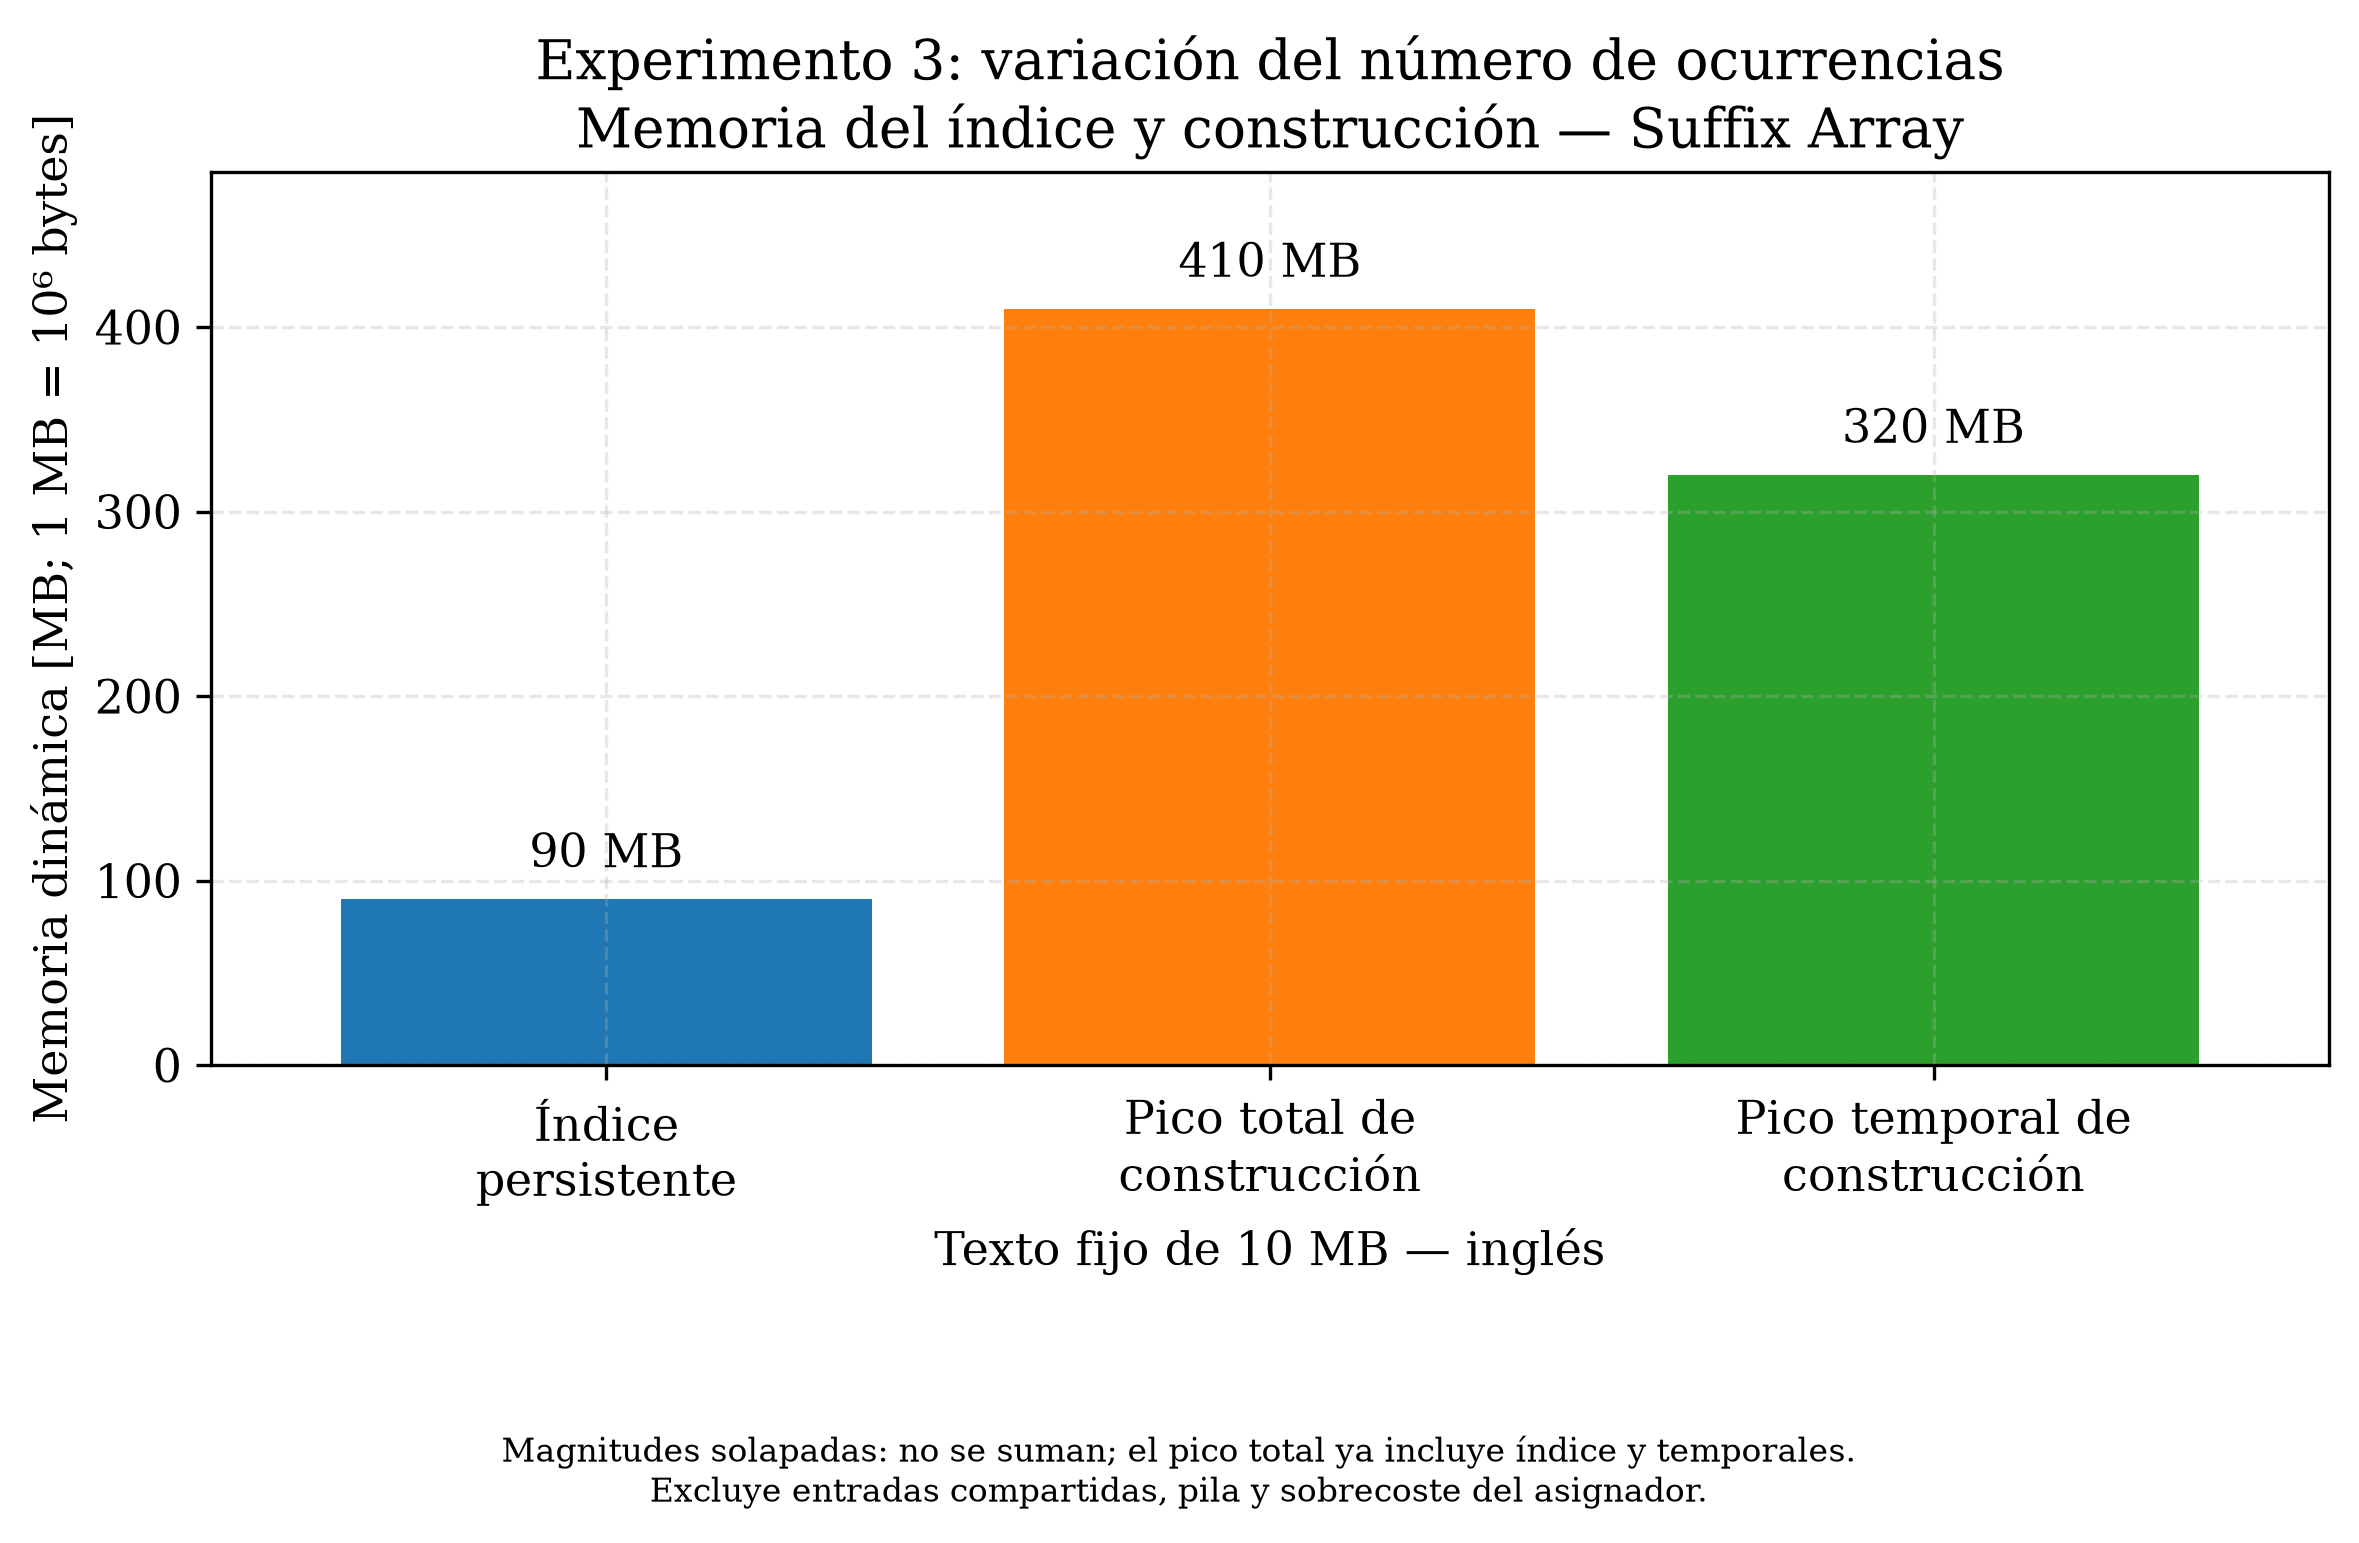
\includegraphics[width=\linewidth]{../plots/experimento_3_numero_ocurrencias/memoria_indice_y_construccion_suffix_array_texto_fijo.png}
        \caption{Memoria del índice y construcción.}
        \label{fig:res-ocurrencias-memoria-indice}
    \end{subfigure}

    \par\medskip
    \begin{subfigure}[t]{0.49\linewidth}
        \centering
        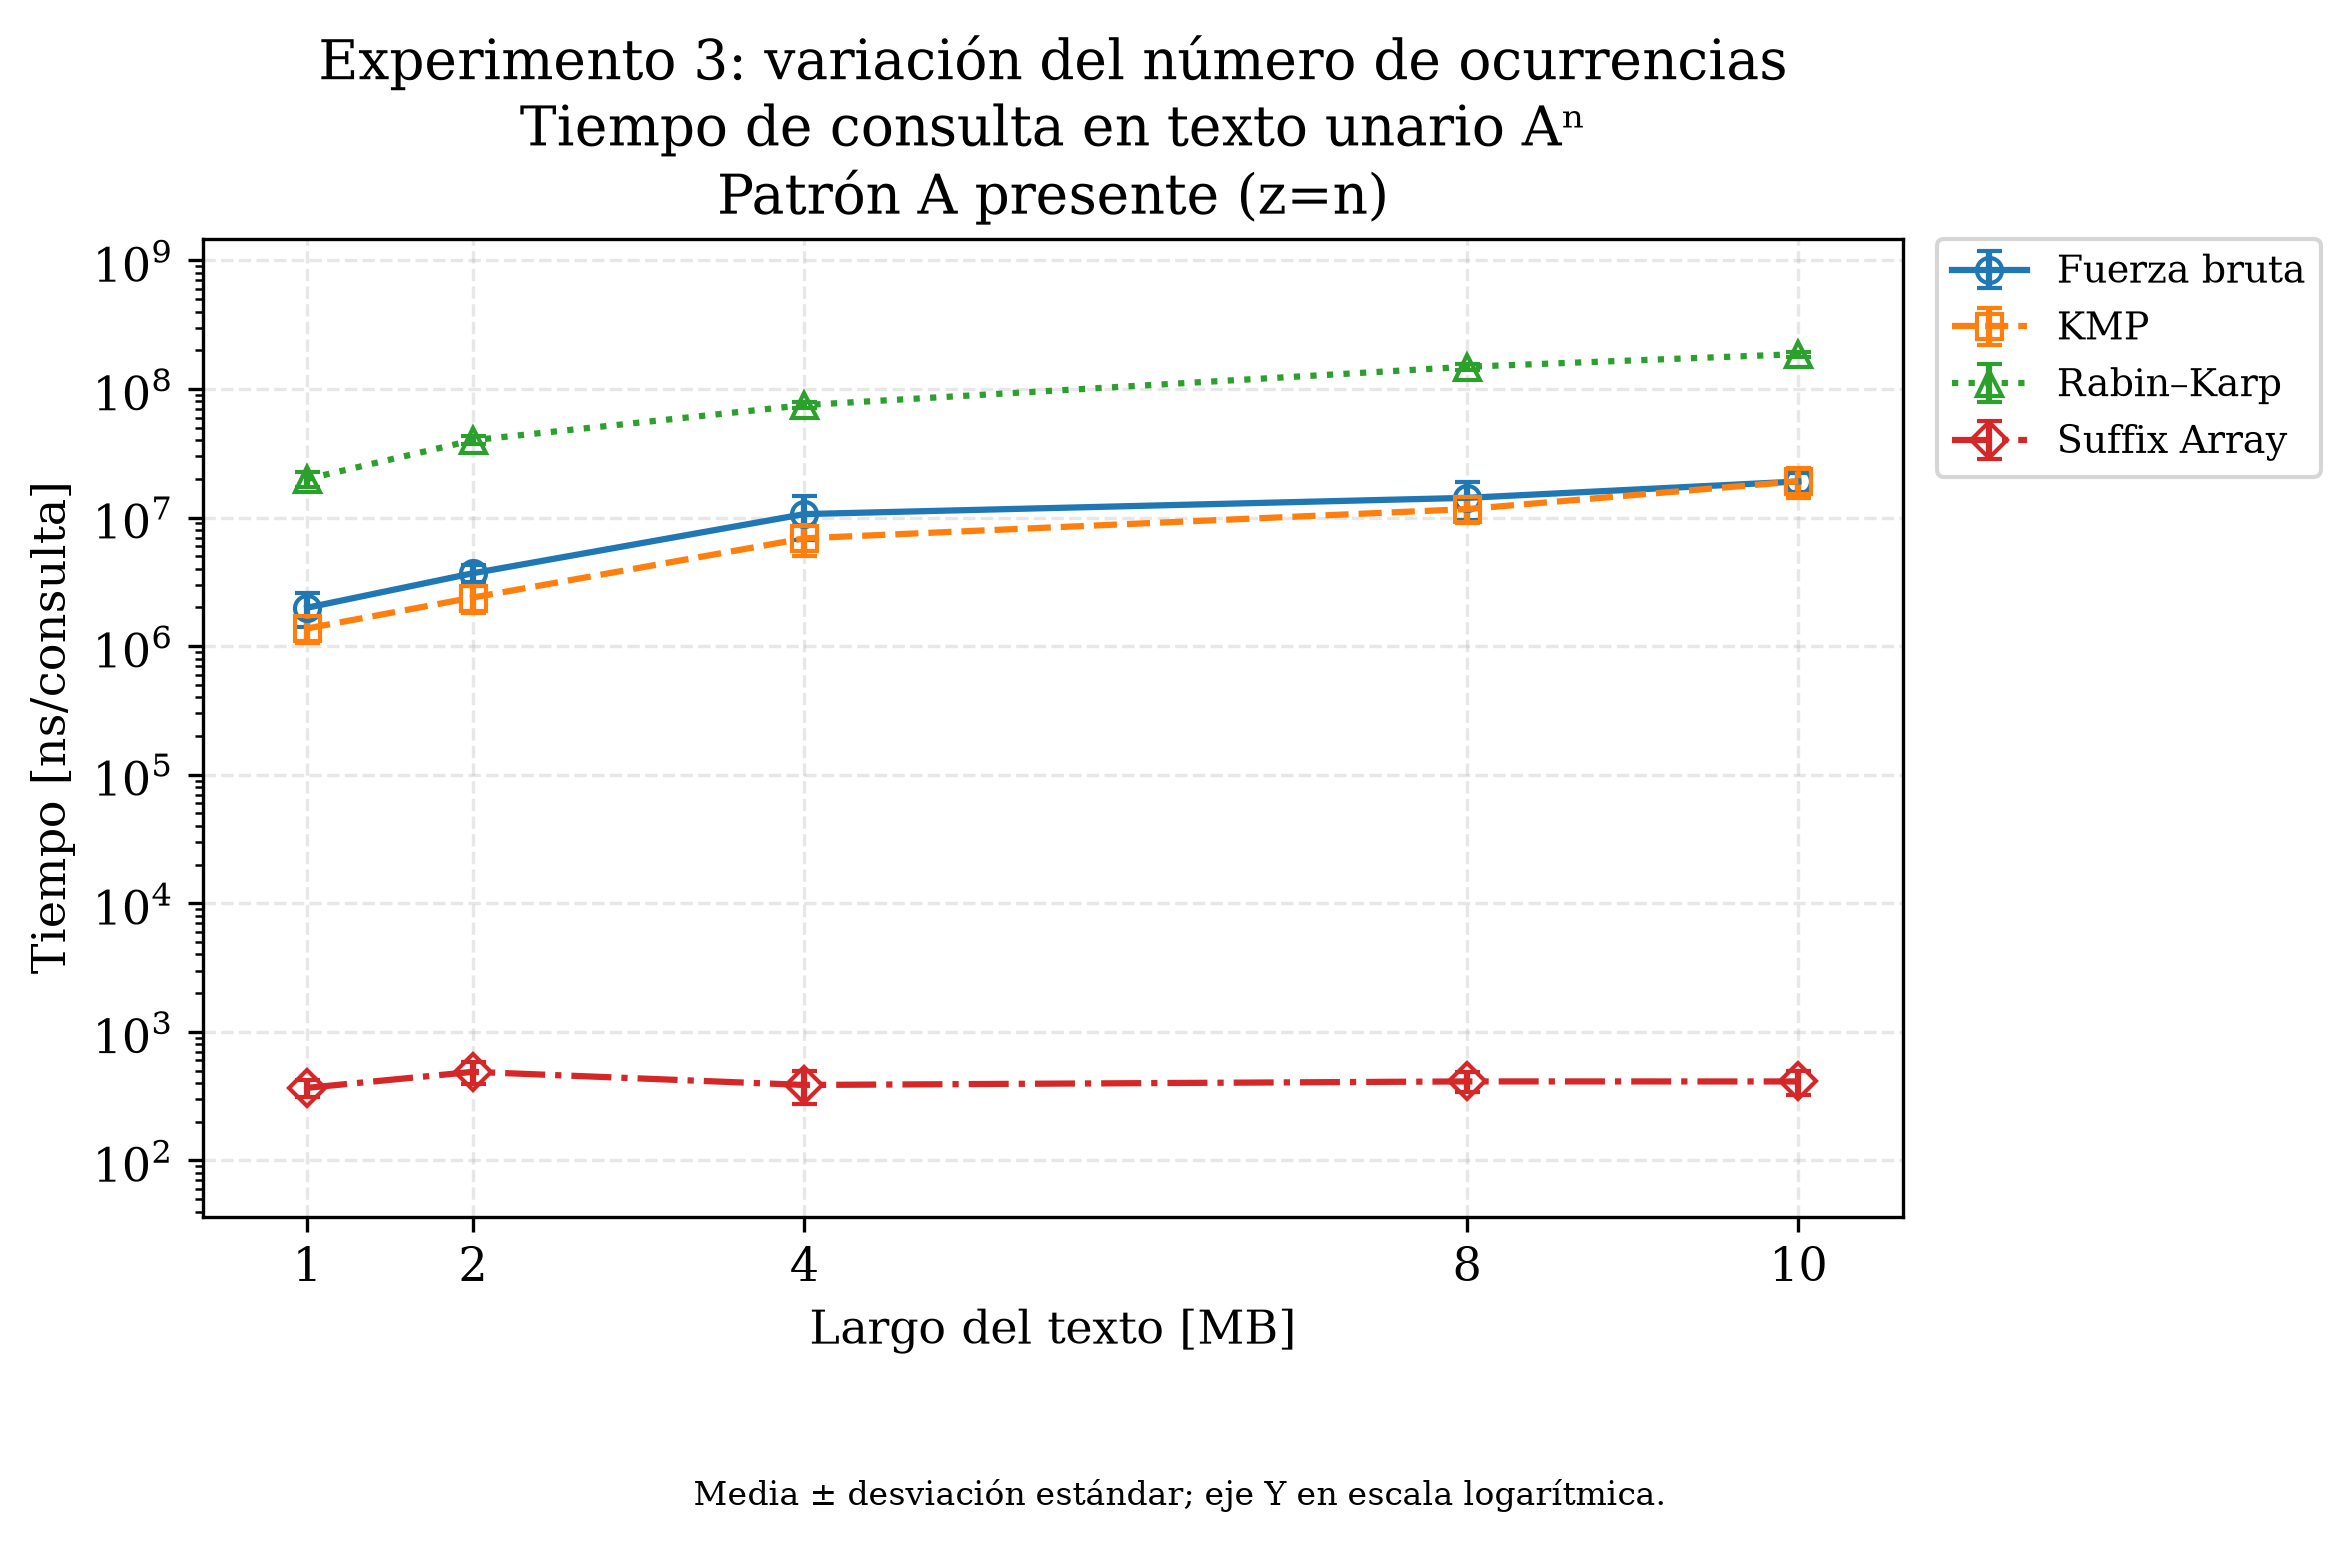
\includegraphics[width=\linewidth]{../plots/experimento_3_numero_ocurrencias/casos_unarios/tiempo_consulta_patron_A_presente_vs_largo_texto.png}
        \caption{Consulta de \(P=A\) en texto unario.}
        \label{fig:res-unario-presente}
    \end{subfigure}\hfill
    \begin{subfigure}[t]{0.49\linewidth}
        \centering
        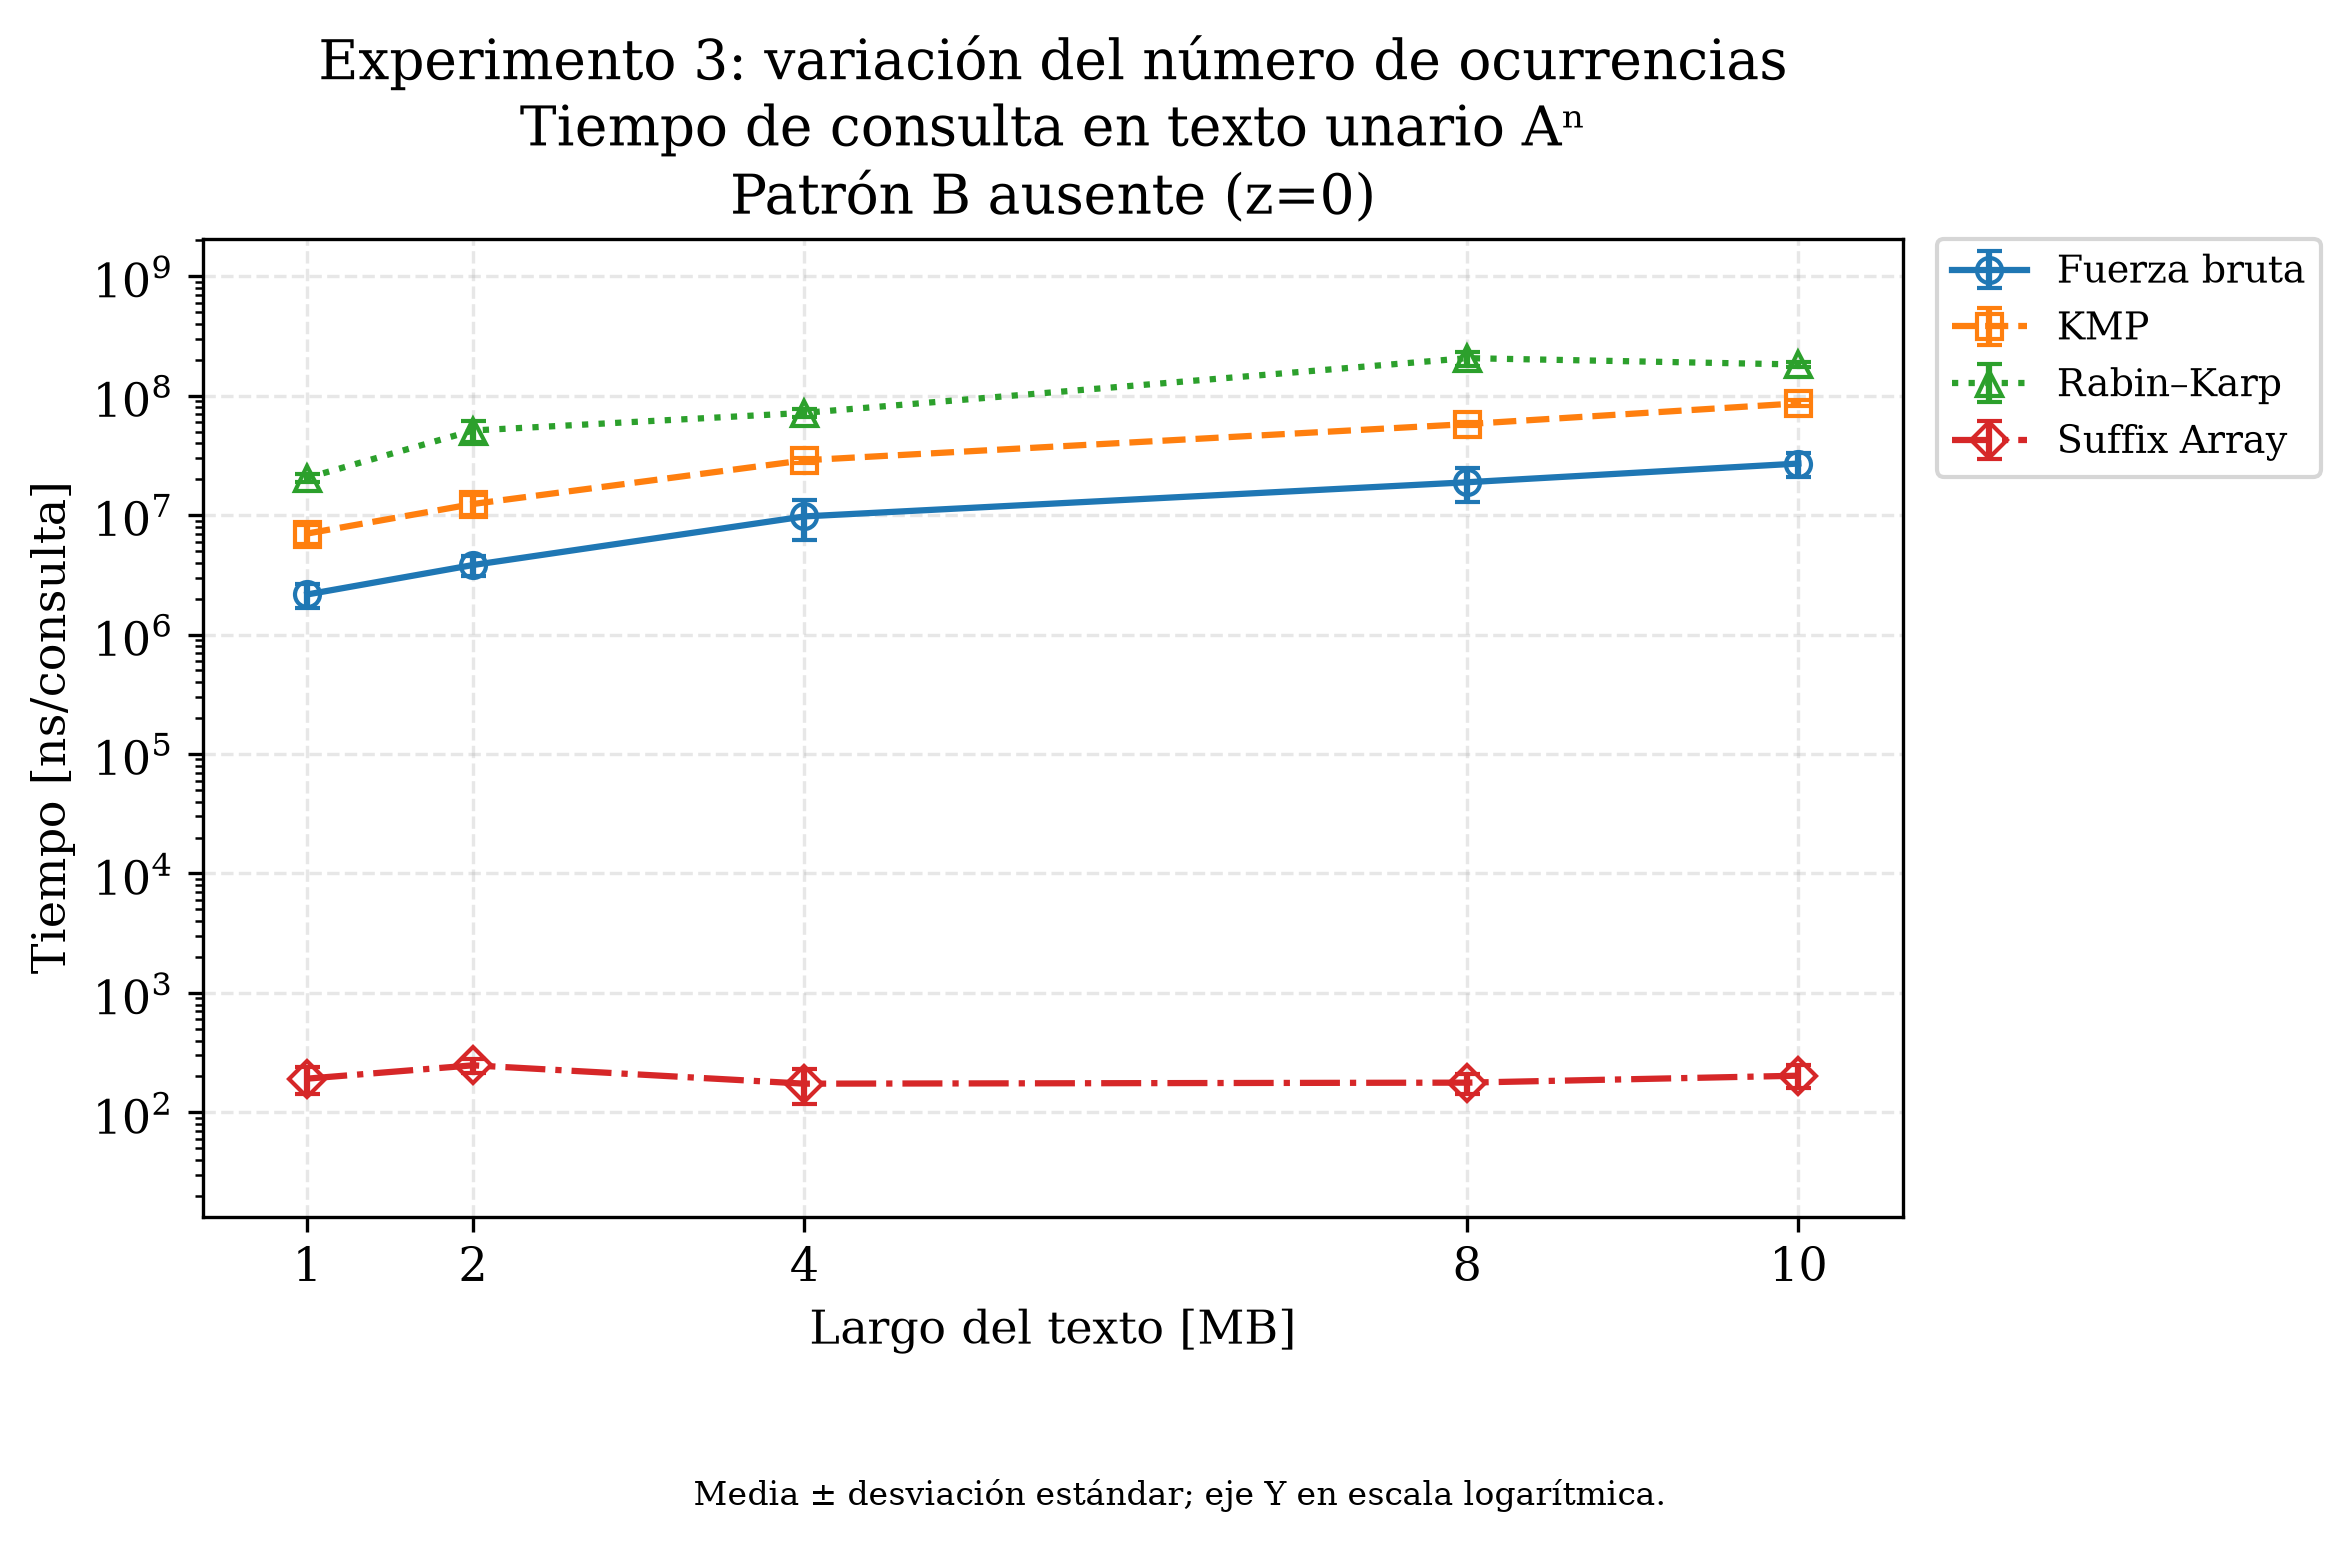
\includegraphics[width=\linewidth]{../plots/experimento_3_numero_ocurrencias/casos_unarios/tiempo_consulta_patron_B_ausente_vs_largo_texto.png}
        \caption{Consulta de \(P=B\) en texto unario.}
        \label{fig:res-unario-ausente}
    \end{subfigure}

    \par\medskip
    \begin{subfigure}[t]{0.54\linewidth}
        \centering
        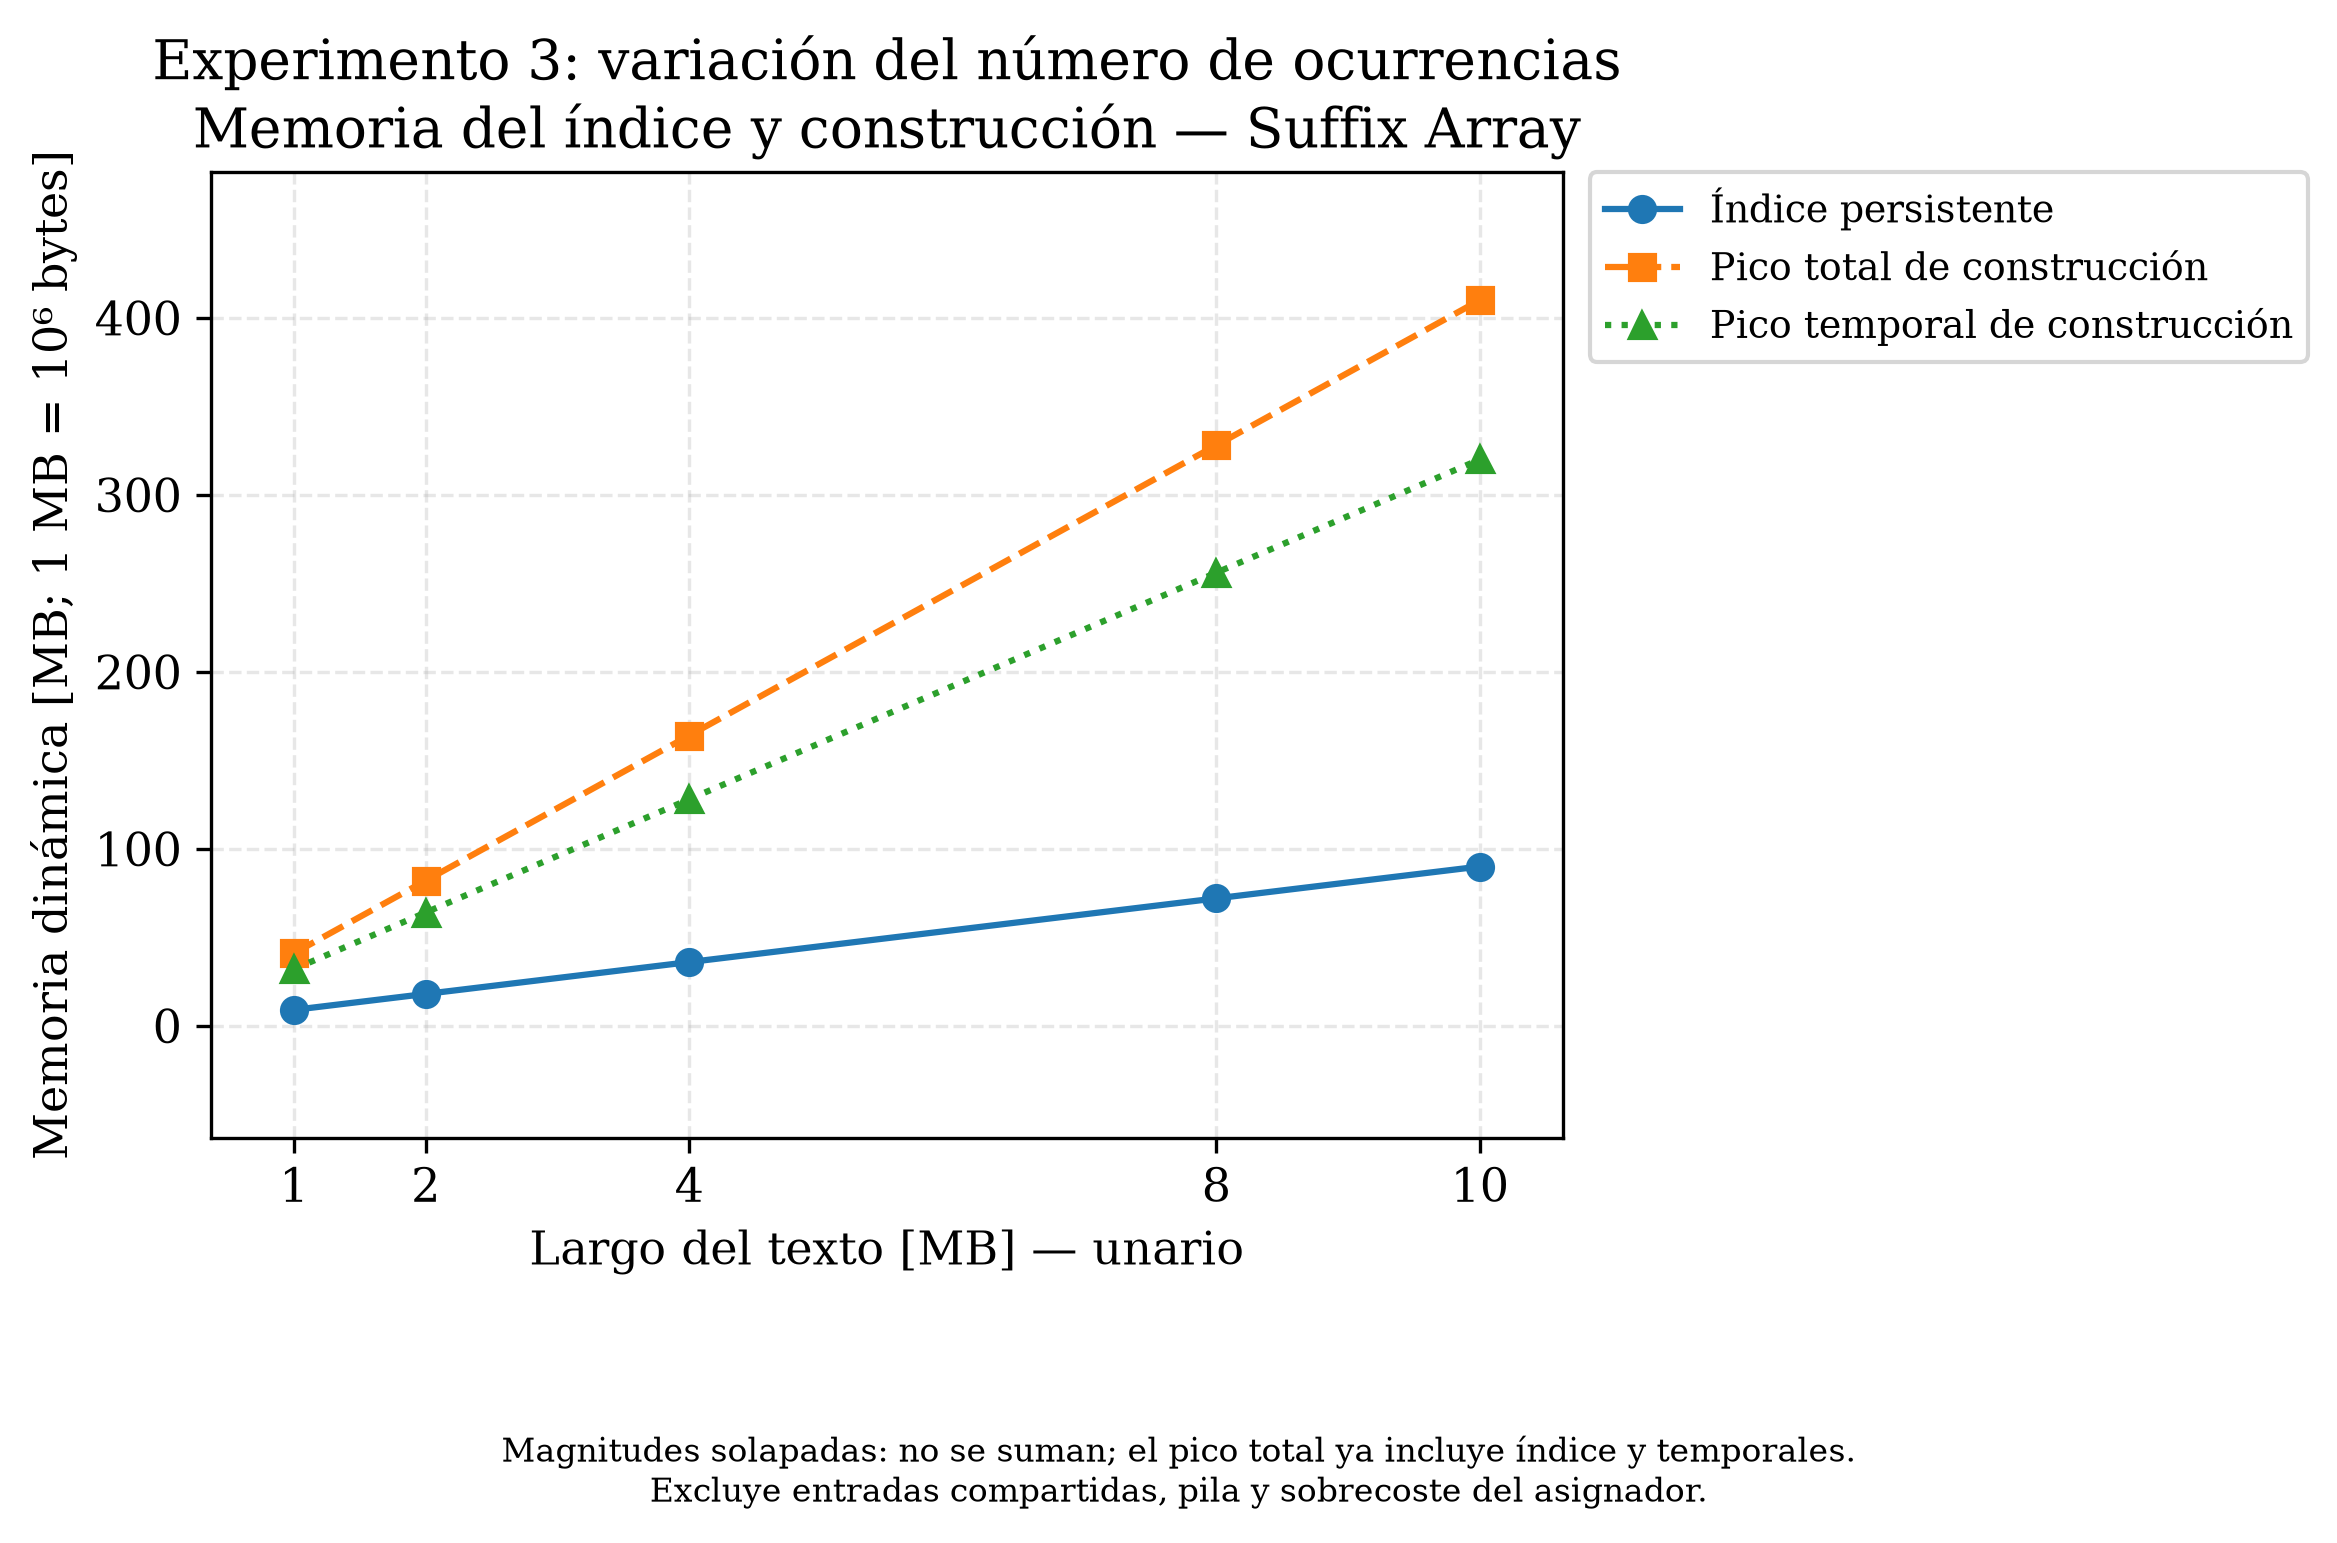
\includegraphics[width=\linewidth]{../plots/experimento_3_numero_ocurrencias/casos_unarios/memoria_indice_y_construccion_suffix_array_vs_largo_texto_unario.png}
        \caption{Memoria del índice para texto unario.}
        \label{fig:res-unario-memoria-indice}
    \end{subfigure}
    \caption{Experimento 3: número de ocurrencias.}
    \label{fig:res-experimento-3}
\end{figure}
\clearpage
% Consultas: data/experimento_{1_largo_texto,2_largo_patron}/plot_summary.csv.
% Construcción: data/experimento_1_largo_texto/{summary,memory}.csv.
% Valores del experimento correspondiente, redondeados después de convertir unidades.
\subsection{Resumen numérico de tiempos y memoria}

Las tablas complementan los gráficos logarítmicos con los valores medidos.
Los tiempos se expresan como media \(\pm\) desviación estándar muestral
de 32 repeticiones; no son intervalos de confianza.

\begingroup
\small
\setlength{\tabcolsep}{4pt}
\renewcommand{\arraystretch}{1.1}

\begin{table}[!ht]
    \centering
    \caption{Consulta según el largo del texto: patrones de 32 bytes y una ocurrencia.}
    \label{tab:res-tiempo-texto}
    \begin{tabular}{@{}rcccc@{}}
        \toprule
        Texto & Fuerza bruta & KMP & Rabin--Karp & Suffix Array \\
        {[MB]} & [ms] & [ms] & [ms] & [\(\mu\)s] \\
        \midrule
        1 & \(3{,}59 \pm 0{,}17\) & \(9{,}38 \pm 0{,}17\) & \(29{,}30 \pm 0{,}99\) & \(0{,}790 \pm 0{,}047\) \\
        2 & \(7{,}80 \pm 0{,}34\) & \(18{,}25 \pm 0{,}25\) & \(46{,}68 \pm 0{,}77\) & \(0{,}685 \pm 0{,}029\) \\
        4 & \(14{,}54 \pm 1{,}23\) & \(42{,}63 \pm 1{,}88\) & \(91{,}52 \pm 1{,}44\) & \(0{,}663 \pm 0{,}044\) \\
        8 & \(21{,}78 \pm 0{,}95\) & \(57{,}60 \pm 1{,}99\) & \(148{,}96 \pm 2{,}63\) & \(0{,}493 \pm 0{,}030\) \\
        10 & \(26{,}47 \pm 2{,}15\) & \(71{,}86 \pm 1{,}95\) & \(227{,}43 \pm 12{,}68\) & \(0{,}532 \pm 0{,}046\) \\
        \bottomrule
    \end{tabular}
\end{table}

\begin{table}[!ht]
    \centering
    \caption{Consulta según el largo del patrón: texto de 10 MB y una ocurrencia.}
    \label{tab:res-tiempo-patron}
    \begin{tabular}{@{}rcccc@{}}
        \toprule
        Patrón & Fuerza bruta & KMP & Rabin--Karp & Suffix Array \\
        {[bytes]} & [ms] & [ms] & [ms] & [\(\mu\)s] \\
        \midrule
        8 & \(46{,}32 \pm 1{,}61\) & \(86{,}75 \pm 2{,}04\) & \(221{,}30 \pm 10{,}67\) & \(0{,}488 \pm 0{,}044\) \\
        16 & \(43{,}37 \pm 1{,}83\) & \(86{,}42 \pm 2{,}37\) & \(187{,}39 \pm 3{,}32\) & \(0{,}537 \pm 0{,}044\) \\
        32 & \(26{,}18 \pm 2{,}20\) & \(72{,}94 \pm 1{,}93\) & \(186{,}65 \pm 4{,}20\) & \(0{,}552 \pm 0{,}043\) \\
        64 & \(47{,}23 \pm 2{,}89\) & \(72{,}34 \pm 1{,}63\) & \(187{,}00 \pm 3{,}23\) & \(0{,}517 \pm 0{,}042\) \\
        128 & \(49{,}24 \pm 2{,}08\) & \(71{,}13 \pm 1{,}79\) & \(188{,}07 \pm 4{,}34\) & \(0{,}509 \pm 0{,}045\) \\
        256 & \(45{,}97 \pm 2{,}26\) & \(71{,}23 \pm 2{,}74\) & \(190{,}37 \pm 4{,}78\) & \(0{,}519 \pm 0{,}043\) \\
        \bottomrule
    \end{tabular}
\end{table}

\begin{table}[!ht]
    \centering
    \caption{Construcción e índice persistente de Suffix Array sobre texto en inglés.}
    \label{tab:res-construccion-memoria}
    \begin{tabular}{@{}rcrr@{}}
        \toprule
        Texto & Construcción & Índice persistente & Pico total de construcción \\
        {[MB]} & [s] & [MB] & [MB] \\
        \midrule
        1 & \(2{,}30 \pm 0{,}12\) & 9{,}00 & 41{,}00 \\
        2 & \(5{,}43 \pm 1{,}02\) & 18{,}00 & 82{,}00 \\
        4 & \(11{,}20 \pm 0{,}74\) & 36{,}00 & 164{,}00 \\
        8 & \(23{,}86 \pm 1{,}97\) & 72{,}00 & 328{,}00 \\
        10 & \(34{,}57 \pm 1{,}94\) & 90{,}00 & 410{,}00 \\
        \bottomrule
    \end{tabular}
\end{table}
\endgroup

\noindent\textit{Notas.} En las dos tablas de consulta se promedian primero,
con igual peso, los cinco patrones de cada configuración dentro de cada
repetición. La desviación estándar describe la variación de esos promedios,
no la dispersión entre patrones. Las consultas de Suffix Array excluyen
la construcción del índice. La memoria se observa en una pasada separada,
sin desviación estándar; cuenta reservas dinámicas, no RSS ni pila.
El pico total ya incluye la memoria persistente presente en ese instante:
no se suman ambas columnas. Se usa \(1\,\mathrm{MB}=10^6\) bytes.

\clearpage

\endgroup
